% !TeX spellcheck = en_GB
%%%%%%%%%%%%%%%%%%%%%%%%%%%%%%%%%%%%%%%%%%
%                                        %
%    Engineer thesis LaTeX template      % 
%                                        %
%%%%%%%%%%%%%%%%%%%%%%%%%%%%%%%%%%%%%%%%%%
%  (c) Krzysztof Simiński, 2018-2022     %
%%%%%%%%%%%%%%%%%%%%%%%%%%%%%%%%%%%%%%%%%%

% compilation:

% pdflatex thesis
% biber    thesis
% pdflatex thesis
% pdflatex thesis 

%%%%%%%%%%%%%%%%%%%%%%%%%%%%%%%%%%%%%%%%%%

\documentclass[a4paper,twoside,12pt]{book}
\usepackage[utf8]{inputenc}                                      
\usepackage[T1]{fontenc}
\usepackage{amsmath,amsfonts,amssymb,amsthm}
\usepackage[polish,british]{babel} 
\usepackage{indentfirst}
\usepackage{lmodern}
\usepackage{graphicx} 
\usepackage{hyperref}
\usepackage{booktabs}
%\usepackage{tikz}
%\usepackage{pgfplots}
\usepackage{mathtools}
\usepackage{geometry}
\usepackage[page]{appendix} 
\usepackage{multirow}


%%% My packages %%%
\usepackage{minted}  
\usepackage{algorithm}
\usepackage{algpseudocode}
\usepackage[framemethod=TikZ]{mdframed}
\usepackage{float}
%%%%%%%%%%%%%%%%%%%%%%%%%%

\usepackage{booktabs}
\usepackage{csquotes}
\usepackage[natbib=true]{biblatex}
\bibliography{bibliography}


\usepackage{setspace}
\onehalfspacing


\frenchspacing

\usepackage{listings}
\lstset{
	language={java},
	basicstyle=\ttfamily,
	keywordstyle=\lst@ifdisplaystyle\color{blue}\fi,
	commentstyle=\color{gray}
}

%%%%%%%%%
 
\mdfsetup{skipabove=0.4mm,skipbelow=0.4mm}
\BeforeBeginEnvironment{minted}{\singlespacing\begin{mdframed}[innertopmargin=0mm, innerbottommargin=0mm, frametitlebelowskip=0pt, frametitleaboveskip=0pt, splittopskip=0pt,linewidth=0.75pt]}
\AfterEndEnvironment{minted}{\end{mdframed}\onehalfspacing}

\BeforeBeginEnvironment{verbatim}{\singlespacing\begin{mdframed}[innertopmargin=1mm, innerbottommargin=1mm, frametitlebelowskip=0pt, frametitleaboveskip=0pt, splittopskip=0pt,linewidth=0.75pt]}
\AfterEndEnvironment{verbatim}{\end{mdframed}\onehalfspacing}

%%%%%%%%%%%% FANCY HEADERS %%%%%%%%%%%%%%%

\usepackage{fancyhdr}
\pagestyle{fancy}
\fancyhf{}
\fancyhead[LO]{\nouppercase{\it\rightmark}}
\fancyhead[RE]{\nouppercase{\it\leftmark}}
\fancyhead[LE,RO]{\it\thepage}


\fancypagestyle{onlyPageNumbers}{%
   \fancyhf{} 
   \fancyhead[LE,RO]{\it\thepage}
}

\fancypagestyle{PageNumbersChapterTitles}{%
   \fancyhf{} 
   \fancyhead[LO]{\nouppercase{\it\rightmark}}
   \fancyhead[RE]{\nouppercase{\it\leftmark}}
   \fancyhead[LE,RO]{\it\thepage}
}


%%%%%%%%%%%%%%%%%%%%%%%%%%%
% listings 
\usepackage{listings}
\lstset{%
language=C++,%
commentstyle=\textit,%
identifierstyle=\textsf,%
keywordstyle=\sffamily\bfseries, %\texttt, %
%captionpos=b,%
tabsize=3,%
frame=lines,%
numbers=left,%
numberstyle=\tiny,%
numbersep=5pt,%
breaklines=true,%
morekeywords={descriptor_gaussian,descriptor,partition,fcm_possibilistic,dataset,my_exception,exception,std,vector},%
escapeinside={@*}{*@},%
%texcl=true, % wylacza tryb verbatim w komentarzach jednolinijkowych
}
%%%%%%%%%%%%%%%%%%%%%%%%%%%%%%%%%%%%

%%%% TODO LIST GENERATOR %%%%%%%%%

\usepackage{color}
\definecolor{brickred}      {cmyk}{0   , 0.89, 0.94, 0.28}

\makeatletter \newcommand \kslistofremarks{\section*{Remarks} \@starttoc{rks}}
  \newcommand\l@uwagas[2]
    {\par\noindent \textbf{#2:} %\parbox{10cm}
{#1}\par} \makeatother


\newcommand{\ksremark}[1]{%
{%\marginpar{\textdbend}
{\color{brickred}{[#1]}}}%
\addcontentsline{rks}{uwagas}{\protect{#1}}%
}

%%%%%%%%%%%%%% END OF TODO LIST GENERATOR %%%%%%%%%%% 

% some issues...

\newcounter{PagesWithoutNumbers}

\newcommand{\hcancel}[1]{%
    \tikz[baseline=(tocancel.base)]{
        \node[inner sep=0pt,outer sep=0pt] (tocancel) {#1};
        \draw[red] (tocancel.south west) -- (tocancel.north east);
    }%
}%

\newcommand{\MonthName}{%
  \ifcase\the\month
  \or January% 1
  \or February% 2
  \or March% 3
  \or April% 4
  \or May% 5
  \or June% 6
  \or July% 7
  \or August% 8
  \or September% 9
  \or October% 10
  \or November% 11
  \or December% 12
  \fi}


%%%%%%%%%%%%%%%%%%%%%%%%%%%%%%%%%%%%%%%%%%%%%%
% Helvetica font macros for the title page:
\newcommand{\headerfont}{\fontfamily{phv}\fontsize{18}{18}\bfseries\scshape\selectfont}
\newcommand{\titlefont}{\fontfamily{phv}\fontsize{18}{18}\selectfont}
\newcommand{\otherfont}{\fontfamily{phv}\fontsize{14}{14}\selectfont}

%%%%%%%%%%%%%%%%%%%%%%%%%%%%%%%%%%%%%%%%%%%%%%
%%%%%%%%%%%%%%%%%%%%%%%%%%%%%%%%%%%%%%%%%%%%%%
%%%%%%%%%%%%%%%%%%%%%%%%%%%%%%%%%%%%%%%%%%%%%%
%%%%%%%%%%%%%%%%%%%%%%%%%%%%%%%%%%%%%%%%%%%%%%
%%%%%%%%%%%%%%%%%%%%%%%%%%%%%%%%%%%%%%%%%%%%%%
%%%%%%%%%%%%%%%%%%%%%%%%%%%%%%%%%%%%%%%%%%%%%%
%%%%%%%%%%%%%%%%%%%%%%%%%%%%%%%%%%%%%%%%%%%%%%
\algnewcommand{\algorithmicand}{\textbf{ and }}
\algnewcommand{\algorithmicor}{\textbf{ or }}
\algnewcommand{\algorithmiceq}{\textbf{ == }}
\algnewcommand{\OR}{\algorithmicor}
\algnewcommand{\AND}{\algorithmicand}
\algnewcommand{\EQ}{\algorithmiceq}
\algnewcommand{\var}{\texttt}


\newcommand{\Author}{Szymon Pluta}
\newcommand{\Supervisor}{Krzysztof Simiński, PhD DSc}
\newcommand{\Consultant}{Name Surname, PhD}
\newcommand{\Title}{Data anonymisation web platform}
\newcommand{\Polsl}{Silesian University of Technology}
\newcommand{\Faculty}{Faculty of Automatic Control, Electronics and Computer Science}
\newcommand{\Programme}{Programme: Informatics}


\addbibresource{bibliography.bib}




\begin{document}
\kslistofremarks
\cleardoublepage
	
%%%%%%%%%%%%%%%%%%  Title page %%%%%%%%%%%%%%%%%%% 
\pagestyle{empty}
{
	\newgeometry{top=2.5cm,%
	             bottom=2.5cm,%
	             left=3cm,
	             right=2.5cm}
	\sffamily
	\rule{0cm}{0cm}
	
	\begin{center}
	
\includegraphics[width=45mm]{logo_eng.jpg}
	\end{center}
	\vspace{1cm}
	\begin{center}
	\headerfont \Polsl
	\end{center}
	\begin{center}
	\headerfont \Faculty
	\end{center}
	\vfill
	\begin{center}
   \headerfont \Programme
	\end{center}
	\vfill
	\begin{center}
	\titlefont Final Project
	\end{center}
	\vfill
	
	\begin{center}
	\otherfont \Title\par
	\end{center}
	
	\vfill
	
	\vfill
	 
	\noindent\vbox
	{
		\hbox{\otherfont author: \Author}
		\vspace{12pt}
		\hbox{\otherfont supervisor: \Supervisor}
	%	\vspace{12pt} % only if applicable; otherwise delete the line
	%	\hbox{\otherfont consultant: \Consultant} % only if applicable; otherwise delete the line
	}
	\vfill 
 
   \begin{center}
   \otherfont Gliwice,  \MonthName\ \the\year
   \end{center}	
	\restoregeometry
}
  

\cleardoublepage
 

\rmfamily
\normalfont



%%%%%%%%%%%%%%%%%% Table of contents %%%%%%%%%%%%%%%%%%%%%%
\pagenumbering{Roman}
\pagestyle{onlyPageNumbers}
\tableofcontents

%%%%%%%%%%%%%%%%%%%%%%%%%%%%%%%%%%%%%%%%%%%%%%%%%%%%%
\setcounter{PagesWithoutNumbers}{\value{page}}
\mainmatter
\pagestyle{empty}

\chapter*{Abstract}
\addcontentsline{toc}{chapter}{Abstract}

1. coraz więcej danych produkowanych
2. które są wykorzystywane przez firmy
3. co sprawia że rośnie istota prywatności danych
4. więc potrzebne są coraz lepsze techniki ochrony danych
5. anonimizacja jest taką metodą ochrony danych
6. więc ją zaimplementuje w sposób ultra generyczny
7. jako nowoczesna web platforma
8. dzięki czemu będzie można ją wykorzystać jako wszechstronne narzędzie dla biznesu i R\&D

\paragraph{Keywords:} 2-5 keywords, separated by commas



\cleardoublepage


\pagestyle{PageNumbersChapterTitles}

%%%%%%%%%%%%%% body of the thesis %%%%%%%%%%%%%%%%%


\chapter{Introduction}

Technological advancement being observed in the past years fundamentally changed the relevance of data in today's digitalized world. Information became an innovation stimulus in the area of research and development. The quantity of data that organizations produce, process, store and share is at a continuous growth. An enormous amount of 1.8 zettabytes ($1.8 \cdot 10^{21}$ bytes) of new data was produced only in the 2011, and every two consecutive years this number is doubling \cite{bib:big_data_security}. After decades of observed technological advancement and innovation, the global internet traffic finally entered the zettabyte-era, as it had reached a magnitude of one zettabyte in 2016, and in the calender month being as early as September \cite{bib:cisco_blog}.

The vast quantities of processed information allowed for brand new research fields such as data science or big data analytics to form, which are used by organizations to derive new insights in a way that was previously impossible. Organizations collect and process the data to enhance the services they provide to the customers through statistical analysis or newly developed computer science processes including data mining and machine learning. The utility of delivered services is increased at a lower cost and improved efficiency through the insights extracted from the collected information about how the services are consumed \cite{bib:anonymization_pipeline}.


\vfill

\footnotesize
\color{blue}
Następne do zrobienia, w uproszczeniu i w podanej kolejności:
\begin{itemize}
\item Jak widać, dane są używane wszędzie. Przeciętna osoba sobie nawet nie zdaje sprawy.
\item Istota prywatności danych, ochrona danych osobowych.
\item Prawo wolno reaguje na uregulowanie ochrony danych osobowych: GDPR dopiero w 2018. Prawo różnie działa w różnych krajach.
\item W czasach narastających danych, dane muszą być zanominizowane, bo...
\item ...ale:
\end{itemize}

\normalsize
\color{black}

\footnotesize
\color{blue}
Wniosek: generyczny sposób anonimizacji - nie ma takiego.

\begin{itemize}
\item Mogą istnieć dobre algorytmy anonimizacji, ale są optymalale jedynie w określonych kontekstach

\item \textbf{Cel pracy}: stworzenie generycznego rozwiązania do anonimizacji baz danych w dowolnej formie danych (nieważne co dane reprezentują).

\item Kontroler danych zna swoje dane i sam dostosowuje optymalny sposób anonimizacji.

\item Rozwiązanie może być dostarczone jako free-access (research), B2C lub nawet B2B.

\item Zakres pracy, opis rozdziałów - na samym końcu, po zrobieniu innych rozdziałów.
\normalsize

\end{itemize}
\color{black}
\normalsize


\begin{itemize}
\item introduction into the problem domain
\item settling of the problem in the domain
\item objective of the thesis 
\item scope of the thesis
\item short description of chapters
\item clear description of contribution of the thesis's author – in case of more authors table with enumeration of contribution of authors
\end{itemize}



\chapter{Problem analysis}

\section{Data explosion}

\subsection{Technology advancement}
The continuous and rapid exponential growth of data being collected globally is further excited by improvements to the overall population's accessibility to the digital technology \cite{bib:big_data_analytics}. Cisco Systems estimates within its annual report \cite{bib:cisco_annual} that 66 percent of the world population will have an access to the web by the 2023, compared to 51 percent in 2018, whereas the number of devices that are connected to the web will reach a staggering value of three times as many as the entire population size – demonstrating a total of 60 percent expansion when compared to 2018. Even the area of mobile connection, which was established long ago, is still sustaining a growth – by 2023, a mobile connectivity will be a privilege for 70 percent of the world's population, compared to 66 percent in 2018. The global average mobile network speeds will be tripled through a rapid increase from 13.2 Mbps in 2018 to 43.9 Mbps in 2023.

\subsection{Data analytics}
Raw representation form of the data is not interpretable until it is put under a context and processed into practical information.
Acquiring relevant insights and conclusions from the information can be achieved through a wide term of analytics, which encompasses the actions needed to be performed to produce new information, including: analysis, filtering, processing, grouping and contextualizing the information. Newly discovered knowledge is inferred from the produced information.
Apart from the processes, analytics also includes the technologies, methodologies and algorithms to use and could be divided into descriptive analytics, diagnostic analytics, prescriptive analytics and predictive analytics \cite{bib:big_data_analytics}.

\subsection{Big data}

Big data analytics deals with the difficulties of managing the observed exponentially increasing collected volumes of data. Its purpose is not only to handle the processing and analysis of the data through specialized software tools and frameworks, but also to handle the means on how this enormous amount of data is collected and stored in the first place. It is in its nature that big data is all about massive volumes of information that require specialized hardware infrastructure to store it \cite{bib:big_data_analytics}.

Services of enterprise organizations are running on all the collected data which can take various forms such as database entries, metrics, logs or outgoing messages. New data streaming technologies working at a large scale needed to be engineered to handle the continuous flow of data between systems and databases. An example of such technology includes Apache Kafka which generates even more than a trillion of messages per day for individual large enterprise organizations taking advantage of it \cite{bib:kafka_online,bib:kafka}.

This only proves that big data deals not only with massive volumes – it has also to deal with the high velocities of data generation, which is yet another characteristic of data \cite{bib:big_data_analytics}. According to DOMO report published back in 2020, 90\% of world's data was generated just in the preceding two years, and on average every person in the world created 1.7 megabytes of data per second – which yields 2.5 quintillion ($2.5 \cdot 10^{18}$) bytes of new data each day \cite{bib:domo}.

The momentum of the immense big data interest growth among organizations is not fading away yet, as more and more new businesses and researches are drawn to this subject. The benefits of big data especially concern scientific organizations and large enterprises of which financial domain and IT industry are the common consumers \cite{bib:anonymization_chaos}. The organizations find the interest in information analytics for remarkably diversified reasons. It is recognized as a field that will entirely alter all parts of civilization such as businesses or society as a whole \cite{bib:big_data_in_practice}.

\subsubsection{Applications}

Various types of organizations collect data to take advantage from the insights derived out of the data. The big data analytics applications' impact can be observed already today in a broad spectrum of domains. 

Leading technology companies, such as Google and Facebook, to name a few, sell anonymised collected user data access to their partner advertisers \cite{bib:big_data_in_practice}. This is legally possible as the information that was anonymised, i.e., de-identified in a way that it is no longer bound to an individual, may flow from a system to a system.

Large Hadron Collider (LHC) located in CERN, being the largest physical experiment, annually produces approximately 30 petabytes of data. LHC takes an advantage of light sensors that monitor the collisions of hundreds of millions of particles accelerated nearly to the speed of light. The collisions create enormous amount of data to be processed by computer algorithms in the hope of discovering new particles, e.g., a Nobel prize awarding discovery of Higgs boson had taken place in 2012 \cite{bib:cern}.

Enterprise stores such as Amazon or SAP Commerce Cloud collect the information regarding the way of how the visitors browse and interact with these stores. Collected information may involve the behavioural data related to customer engagement, such as the pages we visit, event clicks, or the way we scroll the page. The insights derived from the collected information enable making future improvements of these services – for example by improving the digital marketing or performance improvements based on the metrics \cite{bib:sap}. The customer experience is also improved as based on the collected data the advertisements or item recommendations can be tailored to the specific user's preferences. The recommendation engine may also attempt to match your profile data to people of similar profile to provide better recommendations. Services attempt to analyse the behavioural patterns such as time of day we browse the store or what circumstances caused our last visit to finish. Even the details such as the exact neighbourhood location we live in, combined with its estimated wealth, organizations may attempt to guess our potential income level \cite{bib:big_data_in_practice}. These data analytics are performed to improve the possibility of customer buying yet another item.

\section{Data privacy}

The privacy endangerment is inherent to big data and it is its major drawback. Our personal data we continuously give away to third parties is the big data fuel.

As the technology evolves, concerns relating to the privacy of our personal information should also grow – and for a relevant reason.  We tend not to give a second thought to whom the data is shared, how it may be used and in what kind of circumstances. We don't wonder how our own data may be exploited to alter our thinking, decisions, or even ideas – whether in an ethical manner or not. 

Although the use of our personal information existed ever since the very first census was created, data privacy is a relatively new concept, as it did not exist prior to the global adoption of the internet. Granted that our data was used by the researchers even before the digitalized era of the internet, the motives for that usage were not commercial \cite{bib:gdpr_handbook}. Nowadays, the data has most certainly become an asset – a resource like any others, and a rather precious one.

It is argued that the data privacy should be centered only around the data usages that have the potential to be a privacy breach. On the other hand, it is argued that merely a collection of the data is already a privacy harm. The information that was collected is endangered by many threats, including data misuse, data breach, data leak or even authorities accesses without legal obligations. Anonymisation is the best method to mitigate conflicts raised by big data with respect to data privacy and data protection \cite{bib:big_data_privacy}.

Luckily the law had finally caught up to the circumstances of the increasing data usages and the associated risks. New European regulations were adopted in 2018 in the form of General Data Protection Regulation (GDPR) to protect our data privacy in a refined fashion. The data subjects, i.e., the individuals represented by the data \cite{bib:anonymization_pipeline}, now have a better control over their personal information – we are now entitled to know what information concerning us is being  processed and for what purpose. We are also entitled to withdraw at any time the consent for the processing of our data. In case of violations we have the right to complain to authorities and seek justice against both the data controllers, i.e., the entities that determine the intention and means of processing the personal information, and the data processors, i.e., the entities that process the personal information on behalf of the data controllers \cite{bib:gdpr_compliance}.

An overall awareness of the data privacy significance had improved in the society, and the means to achieve the data privacy through data protection had also improved as organizations needed to adopt to the new situation by applying enhanced measures to their protection of data – anonymisation and pseudonymisation being the notable examples of such measures. 

\subsection{Authorization to share data}

Majority of data privacy regulations are based on a consent of an individual, i.e., it is lawful to process and use the information for secondary purposes only if an individual explicitly acknowledge their consent for that \cite{bib:gdpr_practical_guide}. This may appear easier said than done due to the unobvious difficulties data controllers face when trying to obtain such a broad authorization consent that will take into account all possible secondary purpose usages.

Consider a patient entering medical facility for an ordinary appointment. The patient would likely find it unusual, disturbing or even shocking if upon his entrance to the facility he was to receive an overwhelming form that included dozens of independent consent authorization requests. The consents could give the impression of being seemingly unrelated to his visit in the first place, e.g., a constent to share the data with researchers of an university located on another continent. In the end that could destroy the data subject's trust – in this case patient's trust.

This theoretical scenario may not easily be implemented in the real world counterpart, as it could be even impossible to know or predict all possible secondary purpose usages in the first place, and consent based authorization is all about knowing the usages.

Consider a newly discovered purpose to process personal information of an already existing database. Getting a consent after the data had already been collected, i.e., backwards in time, would be impossible to accomplish as the data controller would need to contact potentially hundreds of thousands of people for their explicit consent. New purpose can be discovered years after the data collection.

Having that in mind, no consent is required when processing the data that is already anonymised. A data that was stripped from personal identifying or identifiable information data can be used in any way and can be shared with third parties without previously agreed consent. Data controllers now face a realistic to solve problem of information anonymisation rather than an unrealistic problem of consents collection \cite{bib:anonymizing_health_data}.

It is worth mentioning that there exists cases which are defined under Article 6 of General Data Protection Regulation (GDPR) \cite{bib:art6} when consent is not required to process the data, e.g., if the processing is required to defend the data subject's interests or in order not to break the compliance with legal obligations as a data controller. GDPR is a new European law that replaces the preceeding Data Protection Directive regulation adopted by European Community in 1995 \cite{bib:gdpr_practical_guide}. 

\subsection{General Data Protection Regulation}

One of the primary objectives of GDPR is personal data privacy protection which is a fundamental right and freedom of people as defined under the Recital 1 of GDPR \cite{bib:recital1} and the Charter of Fundamental Rights of the European Union \cite{bib:charter}. Newly discovered challenges for the protection of personal data arise from the ongoing globalization and quick development of digital technologies. This in turn vastly had increased both the scope of the gathering of the data, and the sharing of thereof. General Data Protection Regulation (GDPR) is a data protection law that came into force on May 25, 2018 to addresses these data privacy related issues in a strict manner \cite{bib:recital6}.

Compliance with GDPR law is critical for organizations in the view of significant administrative fines they face. Violations of the data processor and data controller obligations defined in GPDR are subject to costly penalties that are imposed by European authorities. Non compliance with technical rules imply a penalty of 2 percent of the total annual turnover of the previous year, or €10 milion, whichever one is higher, whereas non compliance with basic data protection principles imply an even higher penalty of 4 percent of the total annual turnover of the previous year, or €20 million, whichever one is higher \cite{bib:art83}\cite{bib:gdpr_managing_data_risk}.

Implementation of this law had immediately increased the significance of data anonymisation as an information sanitization process in today's world \cite{bib:anonymization_for_research}. Anonymisation being a specific form of data masking suddenly became more relevant in today's world for the reason that the strict regulations, and therefore administrative fines, defined in GDPR do not apply to the anonymised information. Data protection principles covered throughout GDPR concern only the processing of information that is already identified to a natural person, or that is identifiable to a natural person, i.e., an individual is yet to be identified. Given the fact that anonymised information is by definition not relating to a person, hence it can be completely exempted from falling under the GDPR requirements, which apply only to personal data, as stated under Recital 26 \cite{bib:recital26}:

\begin{displayquote}
	The principles of data protection should apply to any information concerning an identified or identifiable natural person. [\ldots] The principles of data protection should therefore not apply to anonymous information, namely information which does not relate to an identified or identifiable natural person or to personal data rendered anonymous in such a manner that the data subject is not or no longer identifiable. This Regulation does not therefore concern the processing of such anonymous information, including for statistical or research purposes.
\end{displayquote}

GDPR distinguishes personal data, anonymised data and pseudonymised data as distinct variations of data. The information that had gone merely through pseudonymisation process would still fall under the regulations of GDPR, due to the existing relevant possibility of future re-identification of the data subject, whereas in case of the anonymised data, such re-identification is by definition either impossible or extremely impractical, and the anonymisation is irreversible by definition. Anonymised data is completely exempted from being governed by GDPR. Nevertheless, pseudonymisation is still one of many possibilities for the data controllers and data processors to be GDPR compliant \cite{bib:gdpr_practical_guide}. The point of anonymisation in the context of GDPR is to be completely exempted from being governed by this regulation.

\section{Data anonymisation}

The data released by organizations exclude identity related information such as names, addresses, telephone numbers or credit card numbers. Personal data is stripped from disseminated data sets through anonymisation to protect the anonymity of the individuals, i.e., data subjects \cite{bib:anonymization_extensive_study}.

\subsection{Background}
Consider a collection of medical data concerning patients' clinical information. Processing and sharing of medical data volumes is crucial for the evolution of world's healthcare services. Medical researchers and doctors take an advantage of the collected data sets to improve their comprehension of diseases and explore new possibilities to treat these diseases, and hence both the overall capability to treat the diseases and the general efficiency of health services are improved. At last it is the patients who benefit from the research conducted on their data since the services they are offered with continuously improve. Nevertheless, it is known that medical data is exceptionally sensitive by its nature due to the details that include e.g., patient data, laboratory tests results, diagnosis details, prescribed medications and history of diseases \cite{bib:anonymization_emr}.

Having understood how sensitive by its essence is the patient information and the vital needs to share this data, this is where data anonymisation plays an indeed crucial role. It would be impossible to disseminate patient information without prior anonymisation of thereof.

\subsection{Definition}

Anonymisation is a statistical disclosure control method of a particular importance. The ultimate anonymisation goal is to de-identify the data by pruning the personal information in such a way that the relation between data subject and corresponding records is blurred.

The data anonymisation is considered to be an effective one only if both of the following criterias hold true \cite{bib:anonymization_taxa}:
\begin{itemize}
\item performed anonymisation operations are irreversible
\item data subject re-identification is impossible or impractical 
\end{itemize}

\subsection{Data classification}

The prerequisite for anonymisation is to understand the context of what does the data represent and by whom – in addition to how – will it be processed \cite{bib:anonymizing_health_data}. 

The commonly adopted approach when attempting to anonymise the data is to first classify the data attributes as direct identifiers (i.e., personal identifying confidential attributes unique to an individual, such as address or tax identification number), indirect identifiers (i.e., so called quasi-identifiers that when combined can discover the individual's identity – such as sex or date of birth) and non identifiers \cite{bib:privacy_unesco_bigdata,bib:anonymizing_health_data}.

It is context dependent to determine which attributes are quasi-identifiers – and finally which techniques need to be combined to achieve anonymisation. Virtually, even the most unexpected attributes could be quasi-identifiers. Ignoring such fields when preparing for anonymisation may eventually lead to future re-identification of the data subjects, as successfully demonstrated, e.g., when breaking the anonymity of the Netflix Prize dataset back in 2006 \cite{bib:netflix}. Since then significant advancements in the field of de-identification were yielded – and in various domains \cite{bib:netflix_decade_later}.

On the other hand, too much anonymisation of quasi-identifiers strips the data out of utility.

\subsection{Utility trade-off}

The organizations need to compromise between the utility and privacy when releasing the data. As anonymisation level increases when more and more restrictive techniques are applied, the utility of the same data decreases.

Consider the two theoretical boundary cases of either releasing data in its original form which maximizes the utility at the cost of discarding the protection of the data subjects' privacy altogether, and the second case of not releasing any data at all which completely preserves the privacy \cite{bib:privacy_digital_world}.

Clearly the data must not be released in its original state – strict GDPR that imposes large administrative fines \cite{bib:art83} exists to mitigate such violations. On the other hand, data that completely suppresses all the information has no value. The data controllers therefore need to strike a balance between the two cases. An appropriate anonymisation strategy maximizing the utility without endangering the privacy must be adopted.

For this reason the data controllers must select appropriate data masking techniques.

\section{Data masking techniques}

It is not possible to predetermine – in a general fashion and without an extra context – the data masking techniques that need to be combined together in order to achieve an actual anonymisation of the previously identifiable information. Instead, a context consisting of:
\begin{itemize}
	\item exact representation form of the data being processed \textit{(What is the data?)}
	\item data processors who use the data \textit{(Who will use the data?)}
	\item processing purpose, e.g., research objective \textit{(How will the data be used?)}
\end{itemize}
is always required when considering an effective way to anonymise data under that context \cite{bib:anonymizing_health_data}.

\subsection{Suppression}

Suppression is the strongest anonymisation technique which completely removes all the values associated with the given attribute, hence rendering the complete protection of the data and therefore enforcing the best data subjects privacy. It is guaranteed that no further implication attacks can be performed against this data \cite{bib:anonymization_extensive_study}. Nevertheless, suppression being the strongest privacy preserving method implies the highest (i.e., worst) data utility loss as a inseparable consequence – the ultimate cost of complete anonymisation that is to be paid.

Consider the raw data of the three attributes presented in the table \ref{id:tab:suppression_raw} to be put under the process of suppression.

\begin{table}[H]
\centering
\caption{Suppression – input data.}
\label{id:tab:suppression_raw}
\begin{tabular}{ccc}
\toprule
Sex & \multicolumn{1}{l}{PIN codes} & Phone number \\ \midrule
F   & 3248                          & 1212 – 345345  \\
F   & 8090                          & 4000 – 303030  \\
M   & 1337                          & 5191 – 915100 \\
\bottomrule
\end{tabular}
\end{table}

Exemplary results of performed suppression are depicted in the table \ref{id:tab:suppression}. All of the three attributes values were suppressed to the value of the suppression token supplied by the data controller.

\begin{table}[H]
\centering
\caption{Suppression  – masked data.}
\label{id:tab:suppression}
\begin{tabular}{ccc}
\toprule
Sex & PIN codes & Phone number \\ \midrule
F/M & \#\#\#\#  & 3000 – 123123  \\
F/M & \#\#\#\#  & 3000 – 123123  \\
F/M & \#\#\#\#  & 3000 – 123123 \\
\bottomrule
\end{tabular}
\end{table}

Phone number suppression deserves a brief discussion. Consider a context in which an attacker successfully obtained the information of exactly one individual data subject of his interest. Consider that the attacker decided to call the anonymised phone number. This number could be suppressed in a way to specifically protect against this attack and the attacker could call someone intentionally most definitely did not, i.e., data protection officer or authorities. In this scenario it could be trivial to trace the call and find the potential attacker. As demonstrated, suppressed could be used in unobvious ways.

Suppression is typically applied on the column level of an attribute, however it is also applicable to the individual records. When compared to plain generalisation, suppression yields a higher information loss and can be though of as a particular case of generalisation \cite{bib:anonymization_emr}. 

The designed software offers column level suppression with a user specified value (i.e., suppression token). The values are transformed to this user specified value using a simple algorithm shown in Fig. \ref{fig:code:suppression}.

\begin{figure}[H]
\begin{minted}[baselinestretch=1, mathescape, linenos, numbersep=4pt, frame=none, fontsize=\footnotesize, breaklines=true, framesep=1mm]{java}
procedure suppression(values, token)
  for (value in values)
    value := token
  return values
\end{minted}
\caption{Pseudocode – suppression.}
\label{fig:code:suppression}
\end{figure}

\subsection{Generalisation}

Generalisation is the second most common non-perturbative anonymisation technique \cite{bib:privacy_unesco_bigdata}. This technique processes the raw data by aggregating and substituting the initial values of a given attribute to the values that are more general~\cite{bib:privacy_unesco_rule_based}. The process of generalisation constitutes a conversion of any value to a more general scope.

The proposed software solution includes two generalisation strategies, namely:
\begin{itemize}
\item based on the size of distributions
\item based on the number of distributions
\end{itemize}

Consider the raw data of the three attributes presented in the table \ref{id:tab:generalisation_raw} to be put under the process of generalisation.

\begin{table}[H]
\centering
\caption{Generalisation – input data.}
\label{id:tab:generalisation_raw}
\begin{tabular}{@{}cll@{}}
\toprule
\multicolumn{1}{l}{Age} & Salary  & Location    \\ \midrule
27                      & 36 000  & Poland      \\
52                      & 54 000  & Canada      \\
30                      & 180 000 & Poland      \\
68                      & 128 000 & Switzerland \\ \bottomrule
\end{tabular}
\end{table}

Results shown in the table \ref{id:tab:generalisation} include exemplary possible values after being processed by the generalisation method. As depicted in the table, all three attributes have been grouped into broader value ranges, hence undergoing the generalisation, yet every column was generalised with a different generalisation strategy.

\begin{table}[H]
\centering
\caption{Generalised – masked data.}
\label{id:tab:generalisation}
\begin{tabular}{lll}
\toprule
Age   & Salary          & Location      \\ \midrule
26 – 30 & 1 – 60000       & Europe        \\
51 – 55 & 1 – 60000       & North America \\
26 – 30 & 120001 – 180000 & Europe        \\
66 – 70 & 120001 – 180000 & Europe        \\ \bottomrule
\end{tabular}
\end{table}

Age column was generalised with a strategy based on the size of distribution. In this case the size of distribution was defined as 5, as every interval aggregates five distinct increasing integer values.

On the other hand, salary data was generalised with a strategy based on the number of distributions – the values were aggregated to three even distributions.

Finally, the generalisation does not necessarily concern only numerical values as observed in the generalisation of location attribute. To better understand this type of generalisation, consider that the age attribute could be generalised into the values of e.g., \textit{young adult, adult, senior}. This type of generalisation is not supported by the developed software, however an illustration of existence of such method is necessary. The fundamental assumption of the developed software is to be generic, i.e., data context-agnostic, and this generalisation method is too specific in its essence to be implemented in a generic fashion.

Both supported generalisation strategies were further enhanced with customizations. The data processor is allowed to predefine minimum and maximum boundary values for the generalised intervals. The computed starting value for the distribution concerning lowest interval is either minimum raw value or user predefined minimum value, whichever is lower. The maximal value for the highest interval is computed in an analogical way.

\begin{figure}[h]
\begin{minted}[baselinestretch=1, mathescape, linenos, numbersep=4pt, frame=none, fontsize=\footnotesize, breaklines=true, framesep=1mm]{java}
procedure generalise(values, configuration)
  computedMin := min(values.min(), configuration.userMin())
  computedMax := max(values.max(), configuration.userMax())
  distributionSize := configuration.distributionSize()

  // Phase 1: Generate empty intervals.
  intervals := <Interval, Values>
  i := computedMin
  while (i < computedMax)
    interval := asEmptyInterval(i, i + distributionSize)
    insert interval into intervals
    i += distributionSize

  // Phase 2: Populate intervals.
  for (value in values)
    for (interval in intervals)
      if (value is within interval)
        interval := get interval from intervals
        add value to interval
  return intervals
\end{minted}
\caption{Pseudocode – generalisation based on distribution size.}
\label{fig:code:generalisation1}
\end{figure}

The generalisation strategies can be summarized with the pseudocodes shown in Fig. \ref{fig:code:generalisation1} and Fig. \ref{fig:code:generalisation2}.

\begin{figure}[h]
\begin{minted}[baselinestretch=1, mathescape, linenos, numbersep=4pt, frame=none, fontsize=\footnotesize, breaklines=true, framesep=1mm]{java}
procedure generalise(values, configuration)
  computedMin := min(values.min(), configuration.userMin())
  computedMax := max(values.max(), configuration.userMax())
  numberOfDistributions = configuration.numberOfDistributions()

  // Phase 1: Generate empty intervals.
  intervals := <Interval, Values>
  i := computedMin
  
  distributionSize := (computedMax - computedMin) / numberOfDistributions
  j := 0    
  while (j < numberOfDistributions)
    interval := asEmptyInterval(i, i + distributionSize)
    insert interval into intervals
    i += distributionSize
    j += 1

  // Phase 2: Populate intervals.
  for (value in values)
    for (interval in intervals)
      if (value is within interval)
        interval := get interval from intervals
        add value to interval
  return intervals
\end{minted}
\caption{Pseudocode – generalisation based on number of distributions.}
\label{fig:code:generalisation2}
\end{figure}

Generalisation may be applied on a global level or local level \cite{bib:anonymization_extensive_study}. In terms of database related vocabulary, as this paper primarily concerns an anonymisation of databases, we say generalisation on a column or record level, respectively.

\subsection{Perturbation}

Perturbation is a data masking technique which encompasses the process of swapping the original values with artificial ones in a way that the statistical factors of the data are similar to the initial data. Perturbation is typically achieved by adding noise to the information so that the values are slightly different \cite{bib:anonymization_directory_structured}. 

Consider weight and height data shown in the table \ref{id:tab:perturbation_raw}.

\begin{table}[h]
\centering
\caption{Perturbation – input data.}
\label{id:tab:perturbation_raw}
\begin{tabular}{rr}
\toprule
Height & Weight \\ \midrule
166                        & 58                         \\
170                        & 66                         \\
194                        & 91                        \\ \bottomrule
\end{tabular}
\end{table}

The table \ref{id:tab:perturbation} shows the data after it was perturbed using the two different perturbation methods that are supported by the engineered software.

\begin{table}[h]
\centering
\caption{Perturbation – masked data.}
\label{id:tab:perturbation}
\begin{tabular}{rr}
\toprule
Height & Weight \\ \midrule
169                        & 57                         \\
168                        & 67                         \\
193                        & 91                        \\ \bottomrule
\end{tabular}
\end{table}

The supported methods include adding the noise based on the strategies of:
\begin{itemize}
\item fixed value
\item percentage value
\end{itemize}

Height attribute values could have been perturbed using the former (i.e., fixed noise of $\pm 3$), whereas weight attribute values could have been perturbed using the latter (i.e., percentage value of $\pm 5 \%$). In either case, the linkage between individual records is blurred with this technique. 

\begin{figure}[H]
\begin{minted}[baselinestretch=1, mathescape, linenos, numbersep=4pt, frame=none, fontsize=\footnotesize, breaklines=true, framesep=1mm]{java}
procedure perturbation(values, noise)
  for (value in values)
    random := pick random from [value - noise, value + noise] interval
    value := random
    value := fit value within boundaries
  return values
\end{minted}
\caption{Pseudocode – perturbation based on fixed noise.}
\label{fig:code:perturbation_fixed}
\end{figure}

Similarly to generalisation, both perturbation techniques allow the user to explicitly specify the minimum and maximum accepted boundary values.

\begin{figure}[h]
\begin{minted}[baselinestretch=1, mathescape, linenos, numbersep=4pt, frame=none, fontsize=\footnotesize, breaklines=true, framesep=1mm]{java}
procedure perturbation(values, noise)
  for (value in values)
    coeff := pick random from [1 - noise, 1 + noise] interval
    value := value * coeff
    value := fit value within boundaries
  return values
\end{minted}
\caption{Pseudocode – perturbation based on percentage noise.}
\label{fig:code:perturbation_percentage}
\end{figure}

Perturbation technique works the best with continuous values - it is an effective method for de-identification of quasi-identifiers such as dates and numbers \cite{bib:anonymisation_techniques_singapore}. Scientifically advanced perturbation approaches are further divided into linear and non-linear perturbation models \cite{bib:perturbation_methods}.


\subsection{Pattern masking}

Pattern masking is a data distortion technique designed to be used when only some parts of the data should be masked. This technique is typically used to mask e.g., codes of various forms, phone numbers, credit card numbers and other structured data. 

Consider the data shown in the table \ref{id:tab:pattern_masking_raw} to be masked using the patterns from the table \ref{id:tab:pattern_masking_patterns}.

\begin{table}[h]
\centering
\caption{Pattern masking – input data.}
\label{id:tab:pattern_masking_raw}
\begin{tabular}{lll}
\toprule
PIN code & Software version & Product code  \\ \midrule
54850185 & 2.7.1            & BAR/service/1 \\
03013844 & 2.4.0-rc.3       & FOO/service/7 \\
76590209 & 1.0.1-alpha      & QUX/utility/0 \\ \bottomrule
\end{tabular}
\end{table}

\begin{table}[h]
\centering
\caption{Pattern masking – exemplary patterns.}
\label{id:tab:pattern_masking_patterns}
\begin{tabular}{ccc}
\toprule
PIN code & Software version & Product code  \\ \midrule
OOXXXXXO & OOXOX            & UUUOOOOOOOOON \\ \bottomrule
\end{tabular}
\end{table}

Exemplary masked output is shown in the table \ref{id:tab:pattern_masking_masked}.

\begin{table}[h]
\centering
\caption{Pattern masking – masked data.}
\label{id:tab:pattern_masking_masked}
\begin{tabular}{lll}
\toprule
PIN code & Software version & Product code  \\ \midrule
54\verb|#####|5 & 2.0.0 & RAN/service/0 \\
03\verb|#####|4 & 2.7.1 & DOM/service/7 \\
76\verb|#####|9 & 0.1.9 & IZE/utility/1 \\ \bottomrule
\end{tabular}
\end{table}

Analysis of pattern masking possibilities has yielded the need to create a versatile pattern configuration. This technique is therefore highly configurable, i.e., available pattern tokens include: \textit{O} – preserve the character, \textit{X} - mask the character, \textit{U} – mask with random uppercase letter, \textit{L} – mask with random lowercase letter, \textit{N} – mask with random digit, \textit{A} – mask with random alphabetic character and \textit{C} – mask with random alphanumeric character.

User can specify the masking character, e.g., \textit{\#}, and can also decide whether the result is truncated to the pattern length (as shown in the masking of software version in the table \ref{id:tab:pattern_masking_masked}).

\subsection{Hashing}

Hashing is a deterministic masking technique \cite{bib:anonymization_for_research} which transforms the data to the fixed length output. This technique is best used for unstructured data. Available implementations include SHA2 and SHA3.

Consider the server logs depicted in the table \ref{id:tab:hashing_raw}.

\begin{table}[h]
\centering
\caption{Hashing – input data.}
\label{id:tab:hashing_raw}
\begin{tabular}{l}
\toprule
\multicolumn{1}{c}{Server logs} \\ \midrule
185.184.2.198 — 200 POST: /api/v1/auth/refresh-token    \\
185.184.2.198 — 200 POST: /api/v1/worksheets \\
255.7.141.233 — 200 POST: /api/v1/outcomes/generate \\ \bottomrule
\end{tabular}
\end{table}

Exemplary hashed values are located in the table \ref{id:tab:hashing_masked}.

\begin{table}[h]
\centering
\caption{Hashing – masked data.}
\label{id:tab:hashing_masked}
\begin{tabular}{l}
\toprule
\multicolumn{1}{c}{Server logs} \\ \midrule
b27ffd54e5b05a538f333157363f18df0a2aaae5754dfd9ec9daad9cc4ccd7a2 \\
477784538ed600c38f586079a7d5e99aac4af97d1cb322888de54edeb600b14d \\
2cd3e1912285c765f1746d5b68b1fdbbff6be9460e305acc18a1d9d777d89b5e \\ \bottomrule
\end{tabular}
\end{table}

Although a mere inspection of the generated hash value does not immediately trace back to the original value, an attack to de-anonymise the data can be easily performed when the attacker knows what the hashed data represents, e.g. a structured birth date \cite{bib:hash}. Like in the case of all techniques, the decision to use this technique is context dependent.

\subsection{Randomisation}

Randomisation methods offers the best middle ground between maintaining the data utility and preserving the privacy \cite{bib:data_shuffling}. This method can be performed on a column or a row level.

\subsubsection{Column shuffle}

Column shuffle is an exceptionally effective method for breaking the strong links of the data belonging to the individual data subjects. All of that is achieved while preserving the data utility \cite{bib:gdpr_handbook}, hence this technique is great for maintaining the analytical value of the data \cite{bib:data_shuffling}.

Consider the medical data from the table \ref{id:tab:attribute_randomisation_raw}

\begin{table}[h]
\centering
\caption{Randomisation – attribute - input data.}
\label{id:tab:attribute_randomisation_raw}
\begin{tabular}{ll}
\toprule
Identity & Virus        \\ \midrule
John     & Influenza A  \\
Marc     & Pneumonia    \\
Stephen  & Bronchitis   \\ \bottomrule
\end{tabular}
\end{table}

An exemplary randomised data is shown in the table \ref{id:tab:attribute_randomisation_masked}.

\begin{table}[h]
\centering
\caption{Randomisation – attribute – masked data.}
\label{id:tab:attribute_randomisation_masked}
\begin{tabular}{ll}
\toprule
Identity & Virus         \\ \midrule
Stephen  & Pneumonia     \\
Marc     &  Influenza A  \\
John     & Bronchitis    \\ \bottomrule
\end{tabular}
\end{table}

This technique can be used in two ways:
\begin{itemize}
\item shuffle without repetitions which preserves the data distribution
\item shuffle with repetitions which distorts the data distribution
\end{itemize}

\subsubsection{Row shuffle}

The data may also be needed to be shuffled on a record level – similarly, with or without preserving the distribution.

Consider shuffling the characters of an RGB colour described in hexadecimal format. Furthermore, consider a concept of storing a set of abstract decisions (e.g., willingness to participate in the election voting) as a sequence of bits where each bit represents an individual boolean decision. The table \ref{id:tab:record_randomisation_raw} shows the data.

\begin{table}[h]
\centering
\caption{Randomisation – record – input data.}
\label{id:tab:record_randomisation_raw}
\begin{tabular}{lc}
\toprule
Hex triplet & Set of decisions \\ \midrule
FF00FF      & 1101             \\
54E7CD      & 1010             \\
E5E5E5      & 0000             \\ \bottomrule
\end{tabular}
\end{table}

The table \ref{id:tab:record_randomisation_masked} shows the data after the masking process. The colours were processed without preserving the original characters distribution.

\begin{table}[h]
\centering
\caption{Randomisation – record – masked data.}
\label{id:tab:record_randomisation_masked}
\begin{tabular}{lc}
\toprule
Hex triplet & Set of decisions \\ \midrule
0000F0      & 0111             \\
E57DC4      & 1100             \\
5E5555      & 0000             \\ \bottomrule
\end{tabular}
\end{table}


\subsection{Artificial data}

Replacing the original data with an artificial data can be achieved through substitution, tokenisation or random number generation.


\subsubsection{Substitution}

Substitution is of a particular relevance when the masked data needs to be realistic \cite{bib:anonymization_planning}.

Consider the data from the table \ref{id:tab:substitution_raw} undergoing the substitution process.

\begin{table}[h]
\centering
\caption{Substitution – input data.}
\label{id:tab:substitution_raw}
\begin{tabular}{ll}
\toprule
Name   & Surname  \\ \midrule
Jan    & Gold     \\
Bob    & Ng       \\
Bob    & Xi       \\ 
Maria  & Robin    \\ \bottomrule
\end{tabular}
\end{table}

Consider that the data controller provides the following data for the name parameter: \textit{Lucius}, \textit{Decimus}, \textit {Amanda}, and the following data for the surname parameter: \textit{Lucci}, \textit{Rector}. The table \ref{id:tab:substitution_masked} presents an exemplary possible masked result.

\begin{table}[h]
\centering
\caption{Substitution – masked data.}
\label{id:tab:substitution_masked}
\begin{tabular}{ll}
\toprule
Name    & Surname   \\ \midrule
Lucius  & Lucci     \\
Decimus & Rector    \\
Decimus & Lucci     \\ 
Amanda  & Rector    \\ \bottomrule
\end{tabular}
\end{table}

The name attribute is masked without memorylessness, and the masking occurs in a circular manner.

The method is designed to be used with or without memorylessness in mind. Duplicate entries of the same unmasked data values may always be altered to the same masked data values. This technique is also a great extension point for data controller customisations, as the external data set needs to be provided, therefore the data controller can have full control over the data.

\subsubsection{Tokenisation}

In comparison to the substitution technique, this operation is relevant when the masked data does not need to be realistic \cite{bib:anonymization_planning}, i.e., it could be useful to perform the analytics on the frequencies of data duplicates.

Consider the data from a survey question shown in the table \ref{id:tab:tokenisation_raw}.

\begin{table}[h]
\centering
\caption{Tokenisation – input data.}
\label{id:tab:tokenisation_raw}
\begin{tabular}{l}
\toprule
\multicolumn{1}{c}{Survey response} \\ \midrule
Agree                               \\
Not sure                            \\
Agree                               \\
Strongly disagree                   \\ \bottomrule
\end{tabular}
\end{table}

The tokenised data is shown in the table \ref{id:tab:tokenisation_masked}. The \textit{agree} value was tokenised to the same token value hence conserving the frequency characteristics of the data.

\begin{table}[h]
\centering
\caption{Tokenisation – masked data.}
\label{id:tab:tokenisation_masked}
\begin{tabular}{l}
\toprule

\multicolumn{1}{c}{Survey response} \\ \midrule
1                                   \\
2                                   \\
1                                   \\
3                                   \\ \bottomrule
\end{tabular}
\end{table}

\subsubsection{Random number}

The fundamental requirement of anonymisation platform is to be a versatile software to anonymise the data, hence even a simple random number technique needs to be supported to possibly cover a broader range of the business needs.

Consider the data of customer satisfaction described as a value ranging from 1 to 5 shown in the table \ref{id:tab:random_number_raw}.

\begin{table}[H]
\centering
\caption{Random number – input data.}
\label{id:tab:random_number_raw}
\begin{tabular}{c}
\toprule
Customer satisfaction \\ \midrule
2                     \\
1                     \\
3                     \\ \bottomrule
\end{tabular}
\end{table}

The values from the table \ref{id:tab:random_number_masked} show the new masked values.

\begin{table}[H]
\centering
\caption{Random number – masked data.}
\label{id:tab:random_number_masked}
\begin{tabular}{c}
\toprule
Customer satisfaction \\ \midrule
5                     \\
5                     \\
4                     \\ \bottomrule
\end{tabular}
\end{table}


\subsection{Shortening}
Consider the surnames from the table \ref{id:tab:shortening_raw} to be shortened to a length of 5 characters.

\begin{table}[H]
\centering
\caption{Shortening – input data.}
\label{id:tab:shortening_raw}
\begin{tabular}{l}
\toprule
Surname    \\ \midrule
Kowalski   \\
Kowalewski \\
Nowak      \\ \bottomrule
\end{tabular}
\end{table}

The shortened data is visible in the table \ref{id:tab:shortening_masked}.

\begin{table}[H]
\centering
\caption{Shortening – masked data.}
\label{id:tab:shortening_masked}
\begin{tabular}{l}
\toprule
Surname    \\ \midrule
Kowal.     \\
Kowal.     \\
Nowak      \\ \bottomrule
\end{tabular}
\end{table}

It is possible to specify whether or not the each data record should be terminated with a dot.

\section{Existing solutions}

All of the tools have a shared goal of being GDPR compliant in mind. As this section shows, the existing solutions are greatly similar to the engineered software and often offer \textit{less} versatility than the designed anonymisation web platform.

Of course as the data privacy concerns are increasing in the society, the needs for data protection also increase. The relevance of anonymisation will only increase in the future. The market is just not steady yet.

\subsection{Open source software}

\subsubsection{Anonimatron}
Anonimatron is a Java tool designed for anonymisation of the databases specifically for the development purposes. The idea behind the tool is that the software developers may not be authorized to access the production data, yet may be required to reproduce, e.g., data related performance problems. Internally, anonimatron uses the concept of synonyms.


\subsubsection{Anonymizer}
Similarly to Anonimatron, anonymizer is a tool that anonymises the databases specifically for development. This tool was written in Ruby.

\subsubsection{ARX}
ARX is a Java based desktop solution offering a significant variety of advanced data masking techniques. The tool offers a functionality of analysing the usefulness of the generated outcomes.

\subsubsection{Amnesia}
Amnesia is a software system that allows uploading the data, configuring the anonymisation parameters and downloading anonymised outcome. However, it supports merely the text files.


\subsection{Enterprise class software}


\subsubsection{SAP Data Services}
SAP Data Services is an enterprise class data management software which internally uses Data Mask component of the Transformation module to provide the masking functionalities. Data Mask component offers highly configurable functionalities like perturbation, generalisation and pattern masking.

\subsubsection{Oracle Data Masking and Subsetting}
This is a yet another enterprise class data masking software, however it is solely focused on the masking. This software is optimised for Oracle database, however other databases are also partially supported. The available operations include shuffling, randomisation, pattern masking.

\subsubsection{Microsoft Azure ecosystem}
The anonymisation techniques that are used throughout Azure Synapse Analytics, Azure SQL Managed Instance or Azure SQL Database include pattern masking, random number generation and text substitution.

\subsubsection{TurboCat.io}
This tool primarily oscillates between the encryption method to protect the sensitive data.

\section{Anonymisation as a platform}

The people who were software enginers back in 1990s remember how the web had changed everything and how it dominated the marketed and the way business systems are now engineered \cite{bib:clean_architecture}.

The companies started to massively migrate their services to the cloud with the quite recent rise of the containerization and microservice architecture. Trending software concepts such as serverless or event-storming and tools such as Kubernetes — all of them are oscillating around the web, which is really the only clear and technologically available choice to build a new system. All this technological evolvement is enabled by the open source which is also continuously growing together with the web based software systems, in a feedback loop manner \cite{bib:distributed_systems}. The start of the decline in the web's growth is yet to be discovered, and likely will not emerge in the foreseeable future.

With that being said, the designed software system is categorized and delivered as Platform as a Service (PaaS) and runs in the cloud. The fundamental and the most significant objective of the system is to design an innovative platform that will offer anonymisation capabilities through a broad variety of highly configurable anonymisation techniques in such a way that the data controllers can fit their unique business needs easily.

\chapter{Requirements and tools}

\section{Requirements engineering}

\subsection{Functional requirements – domain}

\subsubsection{Data masking}

There should exist data transforming services that will offer the functionalities of the following techniques:
\begin{itemize}
\item suppression
\item generalisation
\item perturbation
\item randomisation
\item tokenisation
\item random number replacement
\item hashing
\item column shuffle
\item row shuffle
\item shortening
\item pattern masking
\end{itemize}

There should be a validation standard established and enforced that will determine if a particular anonymisation technique is compatible with another technique. The techniques should be configurable.

\subsubsection{Starting template generation}

The user should be able to start the generation of a new template based on the database dump file he provides. The acceptable dump files should include compressed archive or plain script file. The user must successfully upload the dump before starting the template generation.

\subsubsection{Template generation progress}

The template generation should involve the sequence of three steps: persisting the dump file, restoring a new database from the dump, extracting metadata about the restored database. The user should be able to view the template generation progress.

This should be presented as a progress panel containing a visualization of three steps. Completion of a step either marks it as a success or error. Currently processing step should be shown. Errors informing about e.g. invalid databases must be reported to the user. The generation progress should internally update status of the template and should be performed as a sequence of events.

\subsubsection{Restore database}

The system should be able to restore a new database from a dump file of either compressed archive or script file.

\subsubsection{Mirror database}

The system should be able to create a mirror of an existing user database. The mirror should be used for writing the anonymisation script into and then dumping into the final outcome result.

\subsubsection{Extract metadata}

The system should extract the metadata from the uploaded database when creating a new template. The metadata must include information concerning the structure of the database, e.g., the tables, columns and primary keys the database contains. Extracted metadata should be persisted in the server database as JSON type. 

\subsubsection{Inspecting metadata}

The user should be able to inspect the extracted metadata.

\subsubsection{Download metadata}

The user should be able to download the extract metadata.

\subsubsection{Viewing templates}

The user should be able to view his templates.

\subsubsection{Producing worksheet}

The user should be able to produce a new worksheet from the templates he created earlier on. Worksheet should be used for building up the anonymisation setup. The worksheet must not be accessible to other users.

\subsubsection{Viewing worksheets}

There should be a table giving an overview of the created worksheets. Only worksheets belonging to the user should be shown. The table should embed buttons to go to viewing the summary or outcome generation.

\subsubsection{Viewing summary}

There should be a summary view which is an overview for the given worksheet. It should contain four distinct sections of information of the worksheet: template section, tables section, operations section and outcomes section.

\subsubsection{Viewing tables}

The tables included in the template should be enlisted in a worksheet summary.

\subsubsection{Adding column operations}

User must have the possibility of adding new anonymisation operations to the anonymisation concerned columns.

\subsubsection{Viewing column operations}

The so far accumulated column operations should be enlisted for each individual database table. Different operations should use different colors to provide a better visualization. Apart from accumulated operations, the view should also show information such as column name, type, nullability or whether the column is a primary or foreign key.

\subsubsection{PK and FK detection}

Primary and foreign keys should be disallowed to undergo anonymisation. An appropriate information to the user should exist to indicate that a given column is primary or foreign key.

\subsubsection{Starting outcome generation}

The user should be able to start the generation of an outcome based on the worksheet he prepared. It should be possible to select compressed archive or script file as a target output for the outcome. Starting the outcome generation must happen in an asynchronous non-blocking way.

On a high level, the outcome generation should include the complex sequential steps of:
\begin{itemize}
\item creating a writeable mirror database of the read-only template database
\item creating a new empty anonymisation script
\item populating the anonymisation script based on the user defined anonymisation setup
\item executing the anonymisation script against the mirror database
\item dumping the anonymised database to the compressed archive or script file
\end{itemize} 

There should be an outcome database entity created with status field. Each consecutive step should update this status. The total time it took to process an outcome should be measured.

\subsubsection{Browsing outcomes}

The user has to have the possibility to browse the outcomes he created in a form of dedicated table. Each outcome should include the status, anonymisation script download button, outcome dump download button. processing time, template name, etc.

\subsubsection{Anonymisation script download}

There should be a way to download an anonymisation script.

\subsubsection{Anonymised dump download}

There should be a way to download an anonymised dump result.

\subsubsection{Account creation}

To create a new account, an anonymous user needs to provide valid information including e-mail address, password and confirmation, name, surname, and optionally the purpose for anonymisation. Creating an account with an e-mail that is already in use must be prohibited. A new account must be verified to access the broad functionalities.

\subsubsection{Account verification}

Upon successful account creation, the user must receive an e-mail with a link to verify the account. User role should change from \textit{unverified} to \textit{verified} due to confirmation.

\subsubsection{Admin verification}

Admin has the means to verify the specified user on his behalf from the users panel.

\subsubsection{Verification expiration}

The verification link that is sent to the user after creating a new account should contain a token that expires after a set amount of time. The system administrator has to have a possibility of runtime configuration of the expiration time.

\subsubsection{User profile}

The user should be able to view and edit his profile details. The user must not be able to change his e-mail address.

\subsubsection{Users panel}

There should be a users panel for the admin to present an overview and manage the users' accounts.

\subsubsection{Block user}

Admin should have the means to block the user from the users panel, effectively disabling the possibility of logging in.

\subsubsection{Unblock user}

Admin will have the means to unblock the blocked user from the users panel, restoring the login capabilities.

\subsubsection{Mark account for removal}

User must be able to initiate the process involving the removal of his account along with all the associated data, hence ensuring GDPR compliance.

The process is started by an explicit user's requests to do so. The system should warn the user with a detailed message and a prompt to type in both the confirmation and the password. If successful, the account is marked for future removal - the account is removed by a dedicated cron-based data pruning service.

\subsubsection{Forcing account removal}

Admin must have the possibility to force the account to be removed in case of urgent needs e.g. due to reasons concerning system security or performance.

\subsubsection{Revert marking account for removal}

A scenario in which user changes his mind to delete his account needs to be supported. The user can revoke his request to remove the account by accessing the link that was earlier sent to his e-mail address.

The revert action should be possible only if all three conditions are met:
\begin{itemize}
\item the link has not yet expired
\item the admin did not explicitly force the account removal
\item the account has not already been removed by the pruning service
\end{itemize}

\subsubsection{Revert account removal expiration}

The undo removal link sent to the user after requesting his account removal contains a token that expires after a set amount of time. The time of exactly how long is the link valid should be determined by the runtime configurable by the system administrator.

\subsubsection{Forgot password}

There should be a way to reset the password that was forgotten. The link should be sent to the user's e-mail address and should be valid only for a configured duration.

\subsubsection{Tasks panel}

There should be a tasks panel for the admin to retrieve and monitor the tasks. The panel should permit a non-blocking on demand execution of the selected individual tasks.


\subsection{Functional requirements – infrastructure}

\subsubsection{Login}

User should be able to login to the system and access his account's resources.

\subsubsection{User context}

The client should know the details of the user who is logged in. There should exist a user context functionality. Upon successful login the information about principal user should be fetched and stored on the client's side in the user context.

\subsubsection{Access token}

A successful authentication should generate an access token which encompasses all the information necessary for the user authentication and authorization. The token should be valid for a brief duration, e.g., 5 minutes – which should be a matter of runtime configuration conducted by the system administrator. The token should be implemented using JSON Web Token (JWT) standard and should be stored on the client's side.

\subsubsection{Refresh Token}

The refresh token which is generated together with access token during authentication should be used to periodically generate a new pair of the access and refresh tokens. There should exist a REST endpoint that will accept current valid refresh token and will output a new access and refresh token - effectively prolonging user's session. This token should be valid for a very long duration, e.g., 6 months – which should be a matter of runtime configuration.

\subsubsection{Logout}

Discarding the access and refresh tokens permits user logout.

\subsubsection{Remember me}

The user should not have to login to his account when starting a new visit unless
\begin{itemize}
\item the refresh token has expired after e.g., 6 months of inactivity
\item the user has cleared browser cache
\item the user is logging from a new device
\end{itemize}

Restarting the anonymisation platform should not logout the user.

\subsubsection{Seamless tokens re-generation}

Axios HTTP client should be configured in such a manner that it will detect a state of expired access token and will seamlessly generate new tokens. When the access token expires, the client should invoke refresh token service to generate a new tokens pairings in such a manner that the user does not even notice this implementation related behaviour. It is required that no unnecessary page refreshes, errors, logouts or prompts to login show up to the user.

\subsubsection{Role-based authorization}

All non-whitelisted REST resources should be protected with a declarative role-based authorization.

\subsubsection{Resources whitelist}

System administrator should be able to configure the REST resources that are whitelisted (i.e., unprotected). These endpoints should not require to be authenticated (i.e., logged in) to access them.

\subsubsection{Redirection}

System should redirect the user to the login page when accessing routes that are non existing or forbidden to access for them.

\subsubsection{Password encryption}

User password should be stored in the database in an ecrypted form using e.g., bcrypt hashing.

\subsubsection{Navigation menu}

The client application should have a navigation menu. The panel should be located on the left side of the screen. Each navigation item should consist of a large icon and a text label. The entire panel should be hideable – the entire page content should seamlessly adapt to this. Optionally, smooth transition animation should be configurable during TypeScript compilation time.

The items should be easily defined, ordered and configured by adopting a standard. Visibility of a particular item must be role-based, e.g. only admin can see \textit{users} item.

\subsubsection{Timestamp data collection}

The system should collect timestamp data about various resources such as users or templates. Some of the data should be client renderable, and some of the data should be merely collected.

Exemplary dates concern:
\begin{itemize}
\item account registration, block, request for removal, removal
\item template generation
\end{itemize}

\subsubsection{Requests data collection}

All HTTP requests to the anonymisation server should be logged in the system. The logged information should include HTTP method, HTTP response status and the request URI.	

\subsubsection{Request validation – client}

The system should disallow sending HTTP requests that fail to meet the validation criterias set with Yup library.

\subsubsection{In-depth validation – client}

Validation rules set by Yup library for the client forms should be enforced by React Hook Forms. 

The client should have the possibility to specify required and optional fields and use custom validation rules such as e-mail or file presence validation.

\subsubsection{Display validation errors}

Client displays validation errors below the concerning HTML inputs.

\subsubsection{Error notifications}

Client uses toast pop-ups to display client and server HTTP errors \cite{bib:rfc7231} – for example 400 Bad Request. The notifications along with the associated message are displayed in the upper-right corner. The pop-ups are red to underline its purpose and the purpose should be further emphasized - by adding more red color – when displaying the errors of extreme importance e.g. database restore failure.

\subsubsection{Success notifications}

Client sent HTTP requests that finished with a successful response \cite{bib:rfc7231} – for example 201 Accepted - should be displayed in a green coloured pop-up along with the associated message.

\subsubsection{Request validation – server}

The system must validate the HTTP requests on the server to protect the system from passing malformed requests sent by the malicious external HTTP clients. The validations should be declaratively used on the Data Transfer Object (DTO) classes. 

Exemplary validation constraints could include checking for values that meet any of the following criterias:
\begin{itemize}
\item not null
\item not blank
\item not empty
\item for integers – of a value in an allowed range
\item for strings – of size in an allowed range
\item non-standard such as e-mail
\end{itemize}

\subsubsection{Maximum file size}

System administrator should be in control of configuration of the maximum accepted sizes of the files sent to the system (i.e. database dumps). The file sizes that are too large must not be accepted.

\subsubsection{In-depth validation – server}

Server should perform numerous other advanced validations specific to individual scenarios.

Exemplary infrastructure related cases should check if:
\begin{itemize}
\item the system is running in cloud environment
\item an entity non compliant with the database schema is trying to be persisted
\item database connection is established
\end{itemize}

Exemplary authorization related cases should check if:
\begin{itemize}
\item user is trying to access another user's resource
\item user is unauthorized to access the resource due to lack of privileges
\item long lasting refresh token has expired
\end{itemize}

Exemplary domain related cases should check if:
\begin{itemize}
\item anonymisation operation is applicable the particular column
\item column is a primary or foreign key
\item a given task is manually executable
\end{itemize}

\subsubsection{Client tables settings}
The tables presented used extensively by the client application should offer the functionalities of:

\begin{itemize}
\item pagination to a set page size
\item filtering by attribute
\item sorting by attribute
\item hiding and showing of columns
\end{itemize}

\subsubsection{File selector}

There should be a custom file selector input that will allow uploading files i.e., database dumps. The component should show the upload progress bar and success or error message upon completion.

\subsubsection{Uniform design}

The user must not be surprised with a particular page looking in an unexpected way. There should be established a uniform design for the client pages. The design should uniformise, e.g., colors, borders, paddings, margins, shadows or components.

\subsubsection{Theme}

The client application should allow an easy way to change the theme colors of the entire application by changing it in one configuration.

\subsubsection{Skeletons and spinners}

The client should use skeletons and spinners to provide a seamless user experience.

\subsubsection{Mail notifications}

The system has the capabilities of sending e-mails notifying about various actions such as expiring account. This functionality should be runtime configurable by the system administrator.

\subsubsection{Database}

The system needs to use a database. The system should not be coupled to a particular database provider.

\subsubsection{Database preloader}

There should be a functionality to preloaded the system with prepared data. A new system instance must include at least one administrator account.

\subsubsection{Dynamic database connection}

There should exist a factory for data sources that will establish a connection to the dynamically created databases restored from dump files uploaded by the users.

\subsubsection{Prune connection pool}

There should be a functionality to drop all existing database connections, effectively allowing to create the database mirrors dynamically.

\subsubsection{Containerization}

Software components of the system should be containerized. All services should be running as containers when running the system in production environment.

\subsubsection{Multiple environments}

The designed system has to be runnable in multiple environments, i.e.:

\begin{itemize}
\item production
\item development
\item development with the \textit{server} profile enabled
\item locally on the host with a database container
\item fully locally on the host
\end{itemize}

\subsubsection{Environment based configuration}

Different environments, i.e., production, develop and local should use different configurations of the environment and anonymisation server.

\subsubsection{Running processes from Java}

There should be the possibility of running external processes such as \textit{psql} directly from the Java code.

\subsubsection{Asynchronous events}

There should be a configuration for handling asynchronous events. The core functionalities of \textit{uploading} and \textit{processing} server modules should be initiated with an asynchronous non-blocking event.

\subsubsection{Scheduling}

There should be a functionality for defining schedulable task services. The services should rely on the cron expression based triggers. Individual tasks should be runtime configurable in terms of their:

\begin{itemize}
\item cron expression
\item whether the task is enabled for automated scheduling
\item whether the task is enabled for manual execution
\item displayed description in the panel
\end{itemize}

\subsubsection{Secrets}

There should be a functionality prepared to load the secrets (i.e., password for the database, JWT secret key, mail service password) from an external file non-published to the public git repository. Continuous Integration related secrets should be configured directly in GitHub.

\subsubsection{SonarQube}

Both the client and the server should be scanned by the SonarQube static analysis tool. This software should be integrated into Quality CI workflow.

\subsubsection{CodeQL}

Application should be scanned by CodeQL for security issues as a part of Security CI workflow.

\subsubsection{Swagger}

The REST API of the anonymisation server is to be documented with Swagger UI.

\subsubsection{File storage}

There should be a way to store the files, i.e., user input dumps, anonymisation scripts, anonymised output dumps (archives, scripts). The files should be stored in grouped directories whose path are runtime configurable. The file names should be randomly picked e.g. as a universally unique identifier (uuid).

\subsubsection{Prune user data}

A service responsible for deleting accounts that were marked for removal should be executed in a periodic manner. Such service should prune the user data. The frequency of how often is the service executed is described as a cron expression. It should be a system administrator runtime configurable property.

\subsubsection{Prune system data}

There should be a script pruning the Docker data from the host system.


\subsection{Non-functional requirements}

\subsubsection{Modular}
Server should be divided into modular architecture where each module has its own responsibiltiy. Modules have to be further divided into layers or packages. System implements client-server architecture.

\subsubsection{Secure}
Achieved through, e.g., vulenarability scanning, token based authentication enhanced with refresh token functionality, client and server validation, containerization, role based endpoint protection.

\subsubsection{Configurable}
System should be highly configurable by the system administrator. The software can be separately configured on the server, client and containers side.

\subsubsection{Confidential}
Data sent by the users should not be accessible by the admins.

\subsubsection{Extensible}
The system should be engineered in a way to be easily extensible with new features such as supporting new database types or new data masking techniques.

\subsubsection{Adaptable}
The system should be able to easily adapt to changing requirements by the means of clean code practices such as modularity and testability.

\subsubsection{Performant}
Achieved through, e.g., using lazy loading of the relations and individual optimisations.

\subsubsection{Responsive}
Achieved through, e.g., performant client routing.

\subsubsection{Engaging}
Achieved by displaying skeletons, spinners and notifications that catch user's attention.

\subsubsection{Usable}
The system features should be easily understandable – the functionalities must not be confusing to be used.

\subsubsection{Testable}
The system code should be written in a testable manner, e.g. by ensuring high quality of the code and separation of concerns.

\subsubsection{Reliable}
Achieved through continuous integration testing and using well known secure libraries.

\subsubsection{User experience}
Achieved through client functionalities such as intuitiveness, responsive design and uniform styling of the system.

\subsubsection{Measurable} 
The system should collect metrics about e.g. processing time of outcomes.

\subsubsection{Modern}
The system must not use obsolete technologies or software engineering design techniques.

\section{System engineering}
\subsection{Use cases}

The use cases were split into two distinct diagrams which group together the use cases concerning:
\begin{itemize}
\item management – shown in Fig. \ref{fig:use_cases_management}
\item anonymisation – shown in Fig. \ref{fig:use_cases_anonymisation} 
\end{itemize}

\begin{figure}
  \centering
  \includegraphics[width=\linewidth]{img/use_cases_core.png}
  \caption{Use cases – core domain}
  \label{fig:use_cases_management}
\end{figure}

\begin{figure}
  \centering
  \includegraphics[width=\linewidth]{img/use_cases_anonymisation.png}
  \caption{Use cases – anonymisation domain}
  \label{fig:use_cases_anonymisation}
\end{figure}

\subsection{REST API}

The communication with the anonymisation server is driven by the RESTful APIs. An overview of the available endpoints is listed in the table \ref{id:tab:rest_api}. The particular endpoint's purpose can be inferred from the surrounding context i.e., requirements, use cases, controller name and the endpoint URI.

\begin{table}[]
\centering
\caption{REST resources – summary.}
\label{id:tab:rest_api}
\begin{tabular}{|c|l|l|}
\hline
\textbf{Controller}                                                & \multicolumn{1}{c|}{\textbf{Type}}   & \multicolumn{1}{c|}{\textbf{Endpoint}} \\ \hline

% Auth
\multicolumn{1}{|c|}{\multirow{2}{*}{Auth}}                        & \multicolumn{1}{l|}{POST}           & /api/v1/auth/login                    \\
\multicolumn{1}{|c|}{}                                             & \multicolumn{1}{l|}{POST}           & /api/v1/auth/refresh-token \\ \hline

%%%%%%%%%%%%%%%%%%
% User
%%%%%%%%%%%%%%%%%%
\multicolumn{1}{|c|}{\multirow{5}{*}{User}}                        & \multicolumn{1}{l|}{GET}            & /api/v1/users\\
\multicolumn{1}{|c|}{}                                             & \multicolumn{1}{l|}{POST}           & /api/v1/users/register \\
\multicolumn{1}{|c|}{}                                             & \multicolumn{1}{l|}{PUT}            & /api/v1/users/{id}/block \\  
\multicolumn{1}{|c|}{}                                             & \multicolumn{1}{l|}{PUT}            & /api/v1/users/{id}/unblock \\ 
\multicolumn{1}{|c|}{}                                             & \multicolumn{1}{l|}{PUT}            & /api/v1/users/{id}/force-removal \\ \hline

%%%%%%%%%%%%%%%%%%
% Verify
%%%%%%%%%%%%%%%%%%
\multicolumn{1}{|c|}{\multirow{3}{*}{Verify}}                      & \multicolumn{1}{l|}{POST}           & /api/v1/users/verify-mail  \\
\multicolumn{1}{|c|}{}                                             & \multicolumn{1}{l|}{POST}           & /api/v1/users/verify-mail/send-again \\
\multicolumn{1}{|c|}{}                                             & \multicolumn{1}{l|}{POST}           & /api/v1/users/\{id\}/confirm-mail-verification \\ \hline

%%%%%%%%%%%%%%%%%%
% ResetPassword
%%%%%%%%%%%%%%%%%%
\multicolumn{1}{|c|}{\multirow{3}{*}{ResetPassword}}               & \multicolumn{1}{l|}{POST}           & /api/v1/reset-password/request-reset  \\
\multicolumn{1}{|c|}{}                                             & \multicolumn{1}{l|}{POST}           & /api/v1/reset-password/change-password \\
\multicolumn{1}{|c|}{}                                             & \multicolumn{1}{l|}{GET}            & /api/v1/reset-password/show-change-password-form \\  \hline

%%%%%%%%%%%%%%%%%%
% Task
%%%%%%%%%%%%%%%%%%
\multicolumn{1}{|c|}{\multirow{2}{*}{Task}}                        & \multicolumn{1}{l|}{GET}            & /api/v1/tasks \\
\multicolumn{1}{|c|}{}                                             & \multicolumn{1}{l|}{POST}           & /api/v1/tasks/\{task\}/execute \\ \hline

%%%%%%%%%%%%%%%%%%
% Template
%%%%%%%%%%%%%%%%%%
\multicolumn{1}{|c|}{\multirow{5}{*}{Template}}                    & \multicolumn{1}{l|}{POST}           & /api/v1/templates  \\
\multicolumn{1}{|c|}{}                                             & \multicolumn{1}{l|}{GET}            & /api/v1/templates/me \\
\multicolumn{1}{|c|}{}                                             & \multicolumn{1}{l|}{GET}            & /api/v1/templates/\{id\}/status \\  
\multicolumn{1}{|c|}{}                                             & \multicolumn{1}{l|}{GET}            & /api/v1/templates/\{id\}/metadata \\ 
\multicolumn{1}{|c|}{}                                             & \multicolumn{1}{l|}{GET}            & /api/v1/templates/\{id\}/dump/download \\ \hline

%%%%%%%%%%%%%%%%%%
% Worksheet
%%%%%%%%%%%%%%%%%%
\multicolumn{1}{|c|}{\multirow{3}{*}{Worksheet}}                   & \multicolumn{1}{l|}{POST}           & /api/v1/worksheets  \\
\multicolumn{1}{|c|}{}                                             & \multicolumn{1}{l|}{GET}            & /api/v1/worksheets/me \\
\multicolumn{1}{|c|}{}                                             & \multicolumn{1}{l|}{GET}            & /api/v1/worksheets/me/\{id\}/summary \\  \hline

%%%%%%%%%%%%%%%%%%
% TableOperation
%%%%%%%%%%%%%%%%%%
\multicolumn{1}{|c|}{TableOperation}                               & \multicolumn{1}{l|}{GET}            & /api/v1/worksheet/\{id\}/table-operations/\{table\}  \\ \hline

% ColumnOperations
\multicolumn{1}{|c|}{\multirow{11}{*}{\footnotesize ColumnOperation}} & \multicolumn{1}{l|}{\footnotesize PUT}                      & \footnotesize /api/v1/worksheet/\{id\}/column-operations/add-suppression.  \\
\multicolumn{1}{|c|}{}                                             & \multicolumn{1}{l|}{\footnotesize PUT}            & \footnotesize /api/v1/worksheet/\{id\}/column-operations/add-generalisati.     \\
\multicolumn{1}{|c|}{}                                             & \multicolumn{1}{l|}{\footnotesize PUT}            & \footnotesize /api/v1/worksheet/\{id\}/column-operations/add-perturbation  \\
\multicolumn{1}{|c|}{}                                             & \multicolumn{1}{l|}{\footnotesize PUT}            & \footnotesize /api/v1/worksheet/\{id\}/column-operations/add-column-shuff.    \\
\multicolumn{1}{|c|}{}                                             & \multicolumn{1}{l|}{\footnotesize PUT}            & \footnotesize /api/v1/worksheet/\{id\}/column-operations/add-hashing         \\
\multicolumn{1}{|c|}{}                                             & \multicolumn{1}{l|}{\footnotesize PUT}            & \footnotesize /api/v1/worksheet/\{id\}/column-operations/add-pattern-mas. \\
\multicolumn{1}{|c|}{}                                             & \multicolumn{1}{l|}{\footnotesize PUT}            & \footnotesize /api/v1/worksheet/\{id\}/column-operations/add-random-num   \\
\multicolumn{1}{|c|}{}                                             & \multicolumn{1}{l|}{\footnotesize PUT}            & \footnotesize /api/v1/worksheet/\{id\}/column-operations/add-row-shuffle     \\
\multicolumn{1}{|c|}{}                                             & \multicolumn{1}{l|}{\footnotesize PUT}            & \footnotesize /api/v1/worksheet/\{id\}/column-operations/add-shortening      \\
\multicolumn{1}{|c|}{}                                             & \multicolumn{1}{l|}{\footnotesize PUT}            & \footnotesize /api/v1/worksheet/\{id\}/column-operations/add-substitution    \\
\multicolumn{1}{|c|}{}                                             & \multicolumn{1}{l|}{\footnotesize PUT}            & \footnotesize /api/v1/worksheet/\{id\}/column-operations/add-tokenization    \\ \hline

%%%%%%%%%%%%%%%%%%
% Outcome
%%%%%%%%%%%%%%%%%%
\multicolumn{1}{|c|}{\multirow{5}{*}{Outcome}}                     & \multicolumn{1}{l|}{POST}           & /api/v1/outcomes/generate  \\
\multicolumn{1}{|c|}{}                                             & \multicolumn{1}{l|}{GET}            & /api/v1/outcomes/me \\
\multicolumn{1}{|c|}{}                                             & \multicolumn{1}{l|}{GET}            & /api/v1/outcomes/\{id\}/status \\  
\multicolumn{1}{|c|}{}                                             & \multicolumn{1}{l|}{GET}            & \footnotesize /api/v1/outcomes/\{id\}/anonymisation-script/download \\ 
\multicolumn{1}{|c|}{}                                             & \multicolumn{1}{l|}{GET}            & /api/v1/outcomes/\{id\}/dump/download \\ \hline

\end{tabular}
\end{table}

\section{Software tools and technologies}

The following listings are presented to give an overview of the designed system in terms of tools and technologies involved to engineer it without diving into the implementation details. This is a brief summary that merely presents the technological landscape of the designed system – should a particular technology receive a greater detail of explanation, e.g., exemplary usage, it will be described in another dedicated unit.

\subsection{Tools}

This section encompasses a summary of tools needed to develop, build, and maintain the system.

\subsubsection{Docker}

Docker is a virtualization software used to develop, run and manage applications in the form of containers taking advantage of Linux kernel features namespaces and cgroups. It consists of three components: the runtime, the daemon engine and the orchaestrator. 

To run the production environment of anonymisation platform, only prior installation of Docker on the host system is required, because containerization technologies like Docker enable a separation of the software from the infrastructure the software is running on \cite{bib:docker_docs}\cite{bib:docker_book}.

\subsubsection{Apache Maven}

Apache Maven is an open source that automates the build process of foremostly Java based projects. Primary Maven objectives include ensuring an easy build process and an uniformly established build system which is achieved through Maven's build lifecycle (i.e., predefined build steps, e.g., \textit{validate}, \textit{compile}, \textit{test} or \textit{install}) \cite{bib:maven_docs}.

Anonymisation platform uses this tool to build the backend server. Maven is put into service in one of the two ways – depending on the selected environment – namely:
\begin{itemize}
\item internally from the Docker container where Maven can be considered as an abstraction that the system administrator does not have be aware of
\item on the host system itself
\end{itemize}

Maven is also used to run the tests. Gradle could be a great alternative to Maven, the choice being preference based in usual scenarios.

\subsubsection{Node.js}

Node.js is a Javascript runtime engine encapsulating V8 engine developed by Google which implements ECMAScript \cite{bib:v8_docs}. While node.js may function as a dedicated backend server, in the case of anonymisation platform it is used merely to build the client application with yarn.

\subsubsection{yarn}

Yet another resource negotiator (yarn for short) is a package manager developed by Facebook, Google and others \cite{bib:yarn_fb}, whose primary purpose is – similarly to \textit{npm} – installation and management of dependencies used by Node.js runtime environment based projects. Yarn also focuses on ensuring high level of security, performance and reliability \cite{bib:yarn_docs}.

While the purpose of Maven is to build and run the backend server, yarn's purpose is to build and run the frontend client application. Consequently, yarn is used in the same way as Maven – either internally in Docker or on the host system – depending on the chosen environment.

\subsubsection{nginx}

Nginx is an open-source that works as a reverse proxy, web server and HTTP load balancer with the first one being the primary function for anonymisation platform. Reverse proxies improve resiliency, security, scalability and performance of the software systems. This is particularly relevant when designing systems that scale horizontally \cite{bib:nginx_cookbook}.

\subsubsection{git}

It's been a while since most developers had already started using git for development, which is the leading software for version control, however not everyone knows it was originally invented by Linus Torvalds specifically for Linux kernel development needs \cite{bib:git_techtalk}. It is clearly necessary to use git during software development due to the essential needs to publish, stash or revert the code changes \cite{bib:git_pro}.

\subsubsection{GitHub Actions}

GitHub Actions is a continuous integration (CI) and continuous delivery (CD) tool that enable creating workflows which automate development processes such as building, testing and deployment of the system.

Developed software uses three distinct workflows to ensure an automation of testing, quality assurance and security resilience.

\subsubsection{SonarQube}

SonarQube is a large scale open-source tool to conduct the code inspection through static analysis methods. This tool platform can reliably detect vulnerabilities, security hotspots, code smells and bugs. 

In the context of designed anonymisation platform, this software is integrated together with Github Actions to ensure quality and security of developed software. Two distinct instances of SonarQube are configured, independently for the client and the server.

\subsubsection{ESLint}

ESLint is yet another tool for static code analysis for JavaScript applications.

It had been necessary to enhance this tool with TypeScript extension in order to successfully integrate it with client application and Github Actions workflow concerning quality.

\subsubsection{Prettier}

For an unified code formatting standard to be established for the client's application, prettier tool which is a modern code formatter was configured within JetBrains Webstorm IDE.

\subsection{Server}

This section encompasses a summary of technologies used for the implementation of modular and REST driven server.

\subsubsection{Java}

Anonymisation server uses the newest long-term support JDK 17 version released in September 2021, although the server is backwards compatible to JDK 11.

Java is still globally the most widely adopted development language \cite{bib:java25years}, even after the 25 years that had passed after its first release – it is a truly mature language, accompanied by all types of frameworks and libraries that one can imagine.

\subsubsection{Spring Framework}

Spring projects can be viewed together as a modular toolkit that addresses the concerns of modern software development \cite{bib:spring_in_action}.

Spring driven software system may include the following Spring projects \cite{bib:spring_docs}:
\begin{itemize}
\item Spring Framework - the core supporting e.g., dependency injection and web applications
\item Spring Boot – to achieve an easier setup of the Spring driven system
\item Spring Data – to retrieve information from databases in a consistent, database-agnostic way
\item Spring Security – to secure the application with authentication and authorization
\end{itemize}

Java based systems typically employ Spring technologies, and so does the anonymisation server, which extensively uses all of the listed above projects. 

\subsubsection{Hibernate}

Hibernate – a JPA implementation – which is a well tested and high performant \cite{bib:hibernate_high_performance} object-relational mapper was a natural choice for the engineered system given the fact that Spring has a built-in support for this library. It is used to map the database entities to the corresponding database tables \cite{bib:hibernate_docs}.

Hibernate functionality was additionally enhanced with Hibernate Types library \cite{bib:hibernate_types} to provide the support for JSON column type – which is not supported by the plain Hibernate but is greatly supported by the underlying PostgreSQL database \cite{bib:postgresql_json}.

\subsubsection{PostgreSQL – Server}

The choice of appropriate database was of particular importance due to domain of the designed system.

PostgreSQL was fourth most popular database management system worldwide back in 2017 as shown in the annual Stack Overflow Developer Survey report \cite{bib:stackoverflow2017}. Each consequtive report demonstrated further growth of PostgreSQL. As PostgreSQL is at continuous growth, MySQL (i.e., the most popular database) is at continuous decline. Latest report published in 2021 \cite{bib:stackoverflow2021} placed PostgreSQL on the second place and it is believed that it will at last beat MySQL this year.

For this reason PostgreSQL was chosen as the database for the server system. This database was also chosen as the supported database type for the data dumps uploaded by data controllers for the purpose of anonymisation.


\subsubsection{PostgreSQL – Client}

PostgreSQL client is installed in the containerized anonymisation server to execute \textit{psql} processes throughout the application's runtime, hence providing the communication capabilities with the potentially remote PostgreSQL server.

The client is used by the ZT Processor Executor library – directly from the Java code.

\subsubsection{ZT Processor Executor}

ZT Process Executor provides capabilities to run external processes directly from the Java code.

This library found many domain-critical applications related to PostgreSQL resources management. The library executes PostgreSQL client processes including:
\begin{itemize}
\item creation of a new database
\item replication of an existing databases
\item database dump restoration
\item anonymisation script execution
\item database dump to script or to archive
\end{itemize}

\subsubsection{JUnit 5}

JUnit 5 is the new and refined version of the worldwide recognized Java testing framework. It is used to drive the unit and integration tests.


\subsubsection{Testcontainers}

Testcontainers is a cutting edge Java library to support instantiation of lightweight Docker containers for the tests needs. Effectively – the tests run in a containerized environment just like the real application hence blurring the technical differences between real and test environments \cite{bib:testcontainers}.

This state-of-the-art library is used by the integration tests to bootstrap the PostgreSQL database for the tests.

\subsubsection{REST Assured}

REST Assured is an integration tests library and a HTTP client which allows sending true HTTP requests to the test server (bootstrapped by Testcontainers library). This library also offers the means to validate received HTTP responses.

The library is used by the integration tests.

\subsubsection{Swagger UI}

One of many Swagger modules is Swagger UI which deals with the design, description and documentation of REST APIs. The library allows visualization and interaction with the API \cite{bib:swagger}.

This library is relevant due to the complexity of the designed system, as it provides the API documentation for the client.

\subsubsection{JJWT}

JSON Web Tokens are required to transport the implemented access and refresh tokens necessary for authentication and authorization purposes. This popular library deals with the creation and validation of the tokens.

\subsubsection{Bouncy Castle}

One of many cryptographic APIs offered by Bouncy Castle library is SHA 3 which internally implements Keccak-f[1600] algorithm.

This library is used by the hashing data masking technique.

\subsubsection{Apache Commons Lang}

The sole purpose of this library is a generation of random alphabetic and alphanumeric characters for pattern masking anonymisation technique.

\subsection{Client}

This section encompasses a summary of technologies used for the implementation of React based client.

\subsubsection{TypeScript}

TypeScript is a transcompiled superset of JavaScript that the developers want to work with the most unless already doing so \cite{bib:stackoverflow2021}. The language was designed by Microsoft to extend JavaScript with types, interfaces and generics.

The language is powering the frontend client application and React.

\subsubsection{React.js}

React.js was the most popular web framework as of 2021 \cite{bib:stackoverflow2021} as it has finally surpassed the obsolete jQuery library. This is an open source library developed by Facebook to build user interfaces for the web. As a high level overview – React centers around the concept of virtual DOM \cite{bib:modern_fullstack}.

\subsubsection{React ecosystem}

Independent authors create many external libraries to drive the React with extended functionalities. React ecosystem is rich in various libraries which typically include \textit{React} word in their names.

Anonymisation client code extensively uses the following popular libraries:
\begin{itemize}
\item React Router – to handle the URL related concepts including routing, navigation and query parameters
\item React Query – as an abstraction and improvement layer for fetching the data
\item React Hook Form – to provide user input validation in the forms based on Yup defined rules
\end{itemize}

\subsubsection{Yup}

Yup is a validation schema builder. In the case of engineered software, the schemas created by Yup are consumed by React Hook Form library to validate the forms.

\subsubsection{Material UI}

Material UI is yet another React library and a large one. This library is responsible for the appearence of the application.

\subsubsection{Axios}

Axios is an asynchronous HTTP client used for sending the requests to the anonymisation server.

\section{Development methodology}

The development was driven by git like in the case of any software project that is of a non-trivial size. A total number of 6XX \textbf{todo} commits\footnote{the data as of 21.01.2022} were pushed to the master branch. Conventional Commits specification was followed in a simplified way.

There were three possible issue types:
\begin{itemize}
\item feature – describing a new functionality
\item improvement – describing an upgrade to the existing functionality
\item epic – describing a big user story that aggregates other issues\cite{bib:agile_essentials}
\end{itemize}

Note that an improvement to the functionality that is still under development is considered a \textit{feature} and not \textit{improvement}.

Furthermore, the labels with the increasing values of \textit{XS}, \textit{S}, \textit{M}, \textit{L} and \textit{XL} were being added to all the tasks upon creation to estimate the time-to-finish complexities. The distribution of the estimations is shown in Fig. \ref{fig:img:estimations}. \textbf{todo updated pie chart}

\begin{figure}
  \centering
  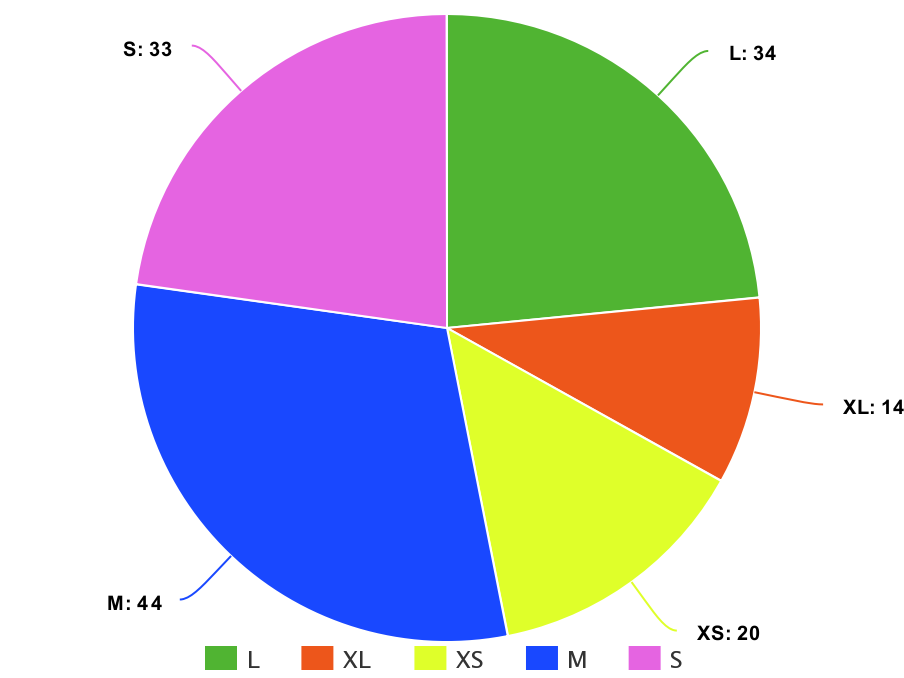
\includegraphics[width=0.65\linewidth]{img/github_issues_sizes.png}
  \caption{GitHub – distribution of tasks estimations.}
  \label{fig:img:estimations}
\end{figure}

The non-epic tasks were marked either as resolved or as cancelled when closing the tasks. Vast majority of tasks was successfully resolved as shown in Fig. \ref{fig:img:resolved_tasks}. Exemplary reasons to close a given task include changing requirements or task duplication.

\begin{figure}
  \centering
  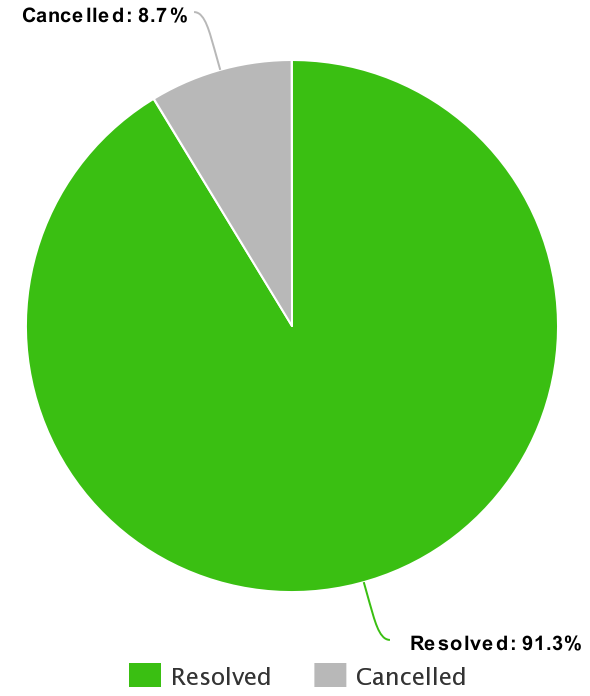
\includegraphics[width=0.5\linewidth]{img/github_issues_finished.png}
  \caption{GitHub – distribution of resolved tasks}
  \label{fig:img:resolved_tasks}
\end{figure}

\subsection{Activation}

New instance of the system database is preloaded with at least one admin account. The credentials of this initial account can be configured from the properties and must be overriden in production:
\begin{verbatim}
core:
  preloader.admin:
    login: admin@admin.com
    password: admin
\end{verbatim}


\subsection{Types of users}

Four types of users can interact with the system:
\begin{itemize}
\item admin user
\item verified user
\item unverified user
\item anonymous user
\end{itemize}

It is very important to note that while the admin user can manage other users accounts, he is not authorized to access the users' confidential data such as anonymisation scripts. The \text{admin user} who may be a non technical business person must not be confused with the \textit{system administrator}.

The relation between the users and their use-cases are summarized in Fig. \ref{fig:use_cases_management} and \ref{fig:use_cases_anonymisation}.

\subsection{System administration}

\chapter{External specification}
\begin{itemize}
\item hardware and software requirements
\item installation procedure
\item activation procedure
\item types of users
\item user manual
\item system administration
\item security issues
\item example of usage
\item working scenarios (with screenshots or output files)
\end{itemize}

\section{Installation}

One of the primary reasons why the containerization concept was so remarkably well received \cite{bib:stackoverflow2021} and exhibited by the massive global adoptions of the Docker technology is the ease it offers regarding the software installation. Decoupling the software from the hardware it runs on allows a portable way to install the software in a simple manner. Instead of making it a responsibility for the end users to manually install the dependent software (e.g., database server, JDK, Node.js or yarn), all the dependencies come encapsulated within the image, effectively transferring the difficulties of managing the dependencies to the application developers.

\subsection{Environments — overview}

The software solution is designed to be runnable in multiple deployment environments hence reproducing the deployment characteristics of a simple modern business-class software system.

As depicted in Fig. \ref{fig:img:environments} the available environments include:
\begin{itemize}
\item production
\item development
\end{itemize}

and the environments are further divided into three available setup options, i.e.:
\begin{itemize}
\item cloud setup
\item semi-cloud setup
\item local setup
\end{itemize}

\begin{figure}[H]
  \centering
  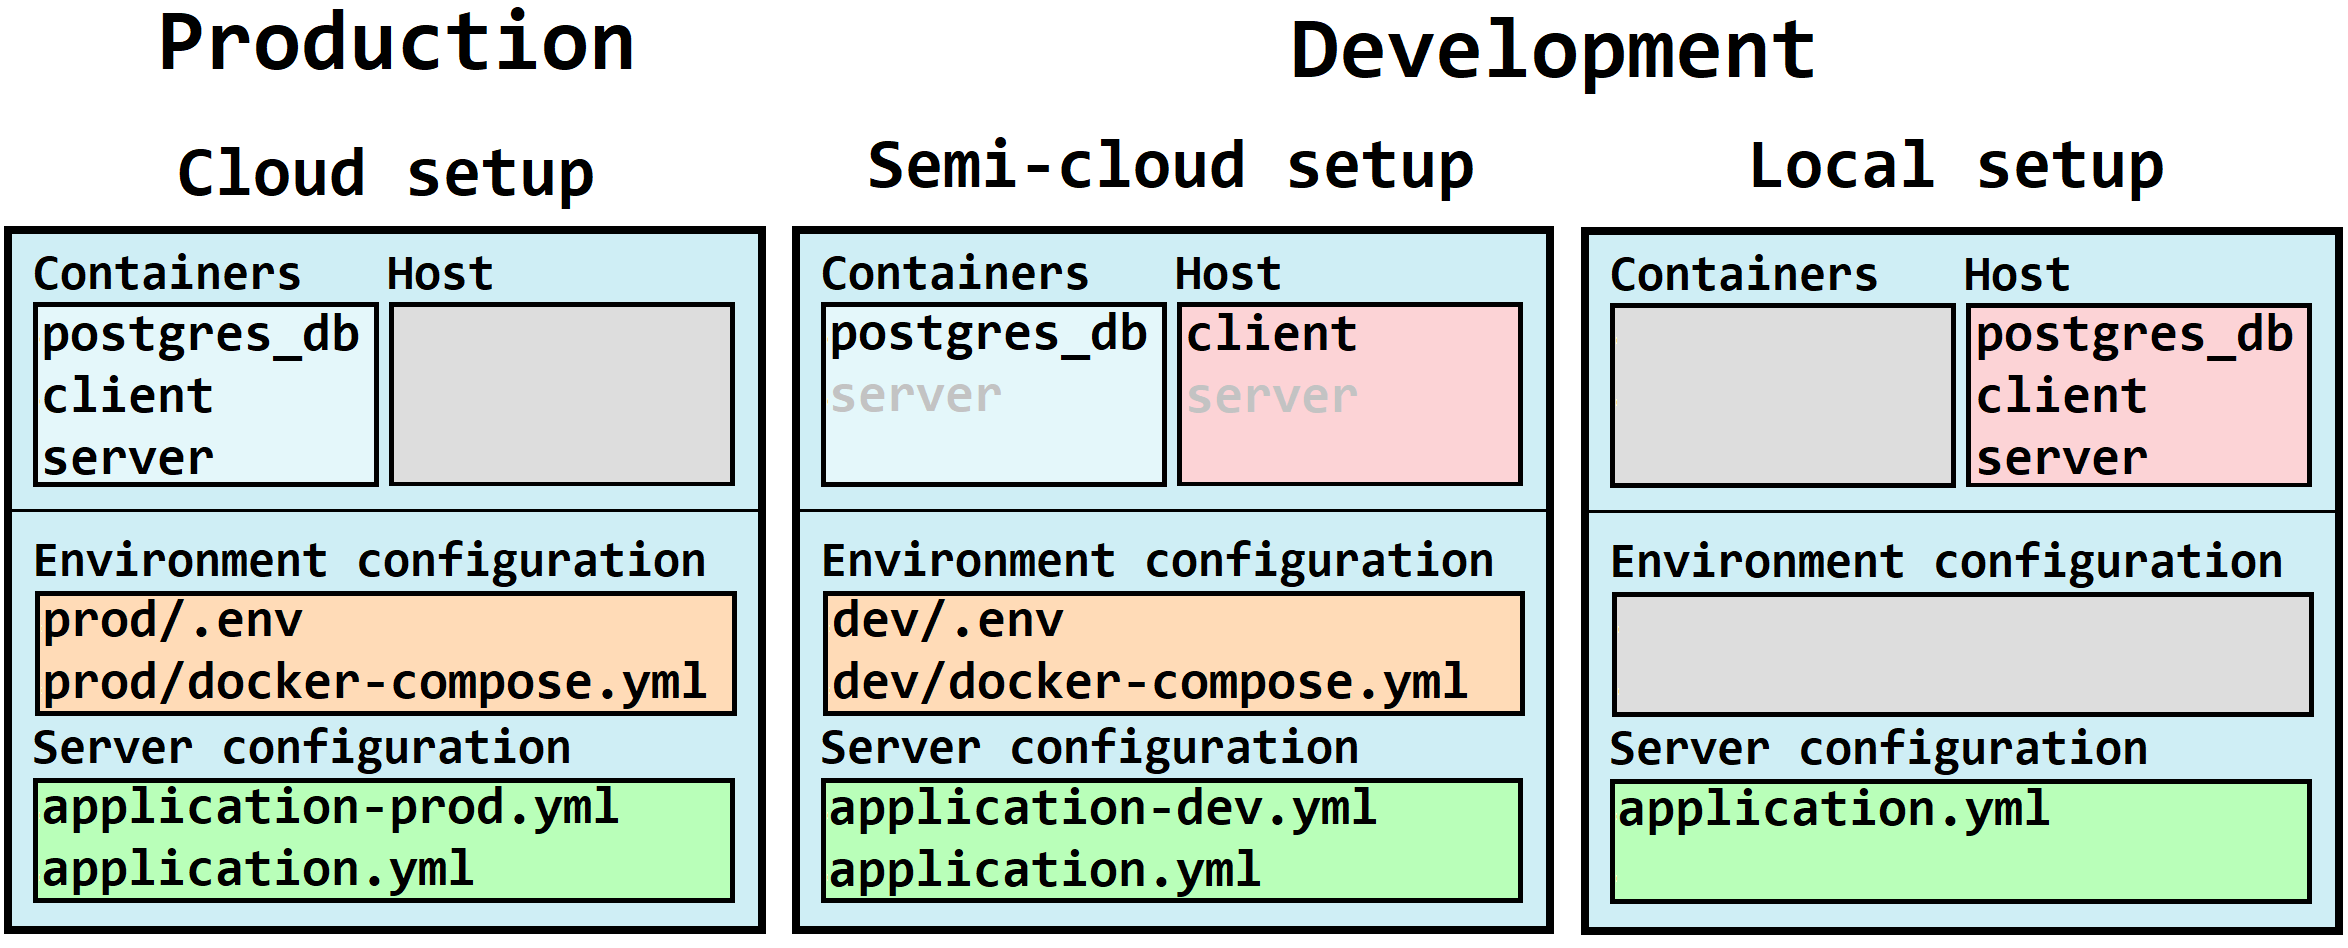
\includegraphics[width=\linewidth]{img/environments.png}
  \caption{Environments}
  \label{fig:img:environments}
\end{figure}

The shared prerequisite for the cloud and semi-cloud setup is to have Docker up and running on the host system. Furthermore, the development environments Local setup does require the installation of additional dependencies.

\subsection{Cloud setup}

The cloud-ready production environment is the easiest one to install.

\subsubsection{Prerequisite}

Docker up and running.

\subsubsection{Installation procedure}

Start up everything at once:

\begin{verbatim}
cd docker/prod
docker compose up
\end{verbatim}

If successful the application should be accessible at \verb|http://localhost:3000|.

The setup is customized from:
\begin{itemize}
\item \verb|prod/.env|
\item \verb|application.yml|
\item \verb|application-prod.yml|
\end{itemize}


\subsection{Semi-cloud setup}

This is the preferred setup for development. PostgreSQL \textit{server} is abstracted away from the host thanks to this setup. Optionally, the anonymisation server can also run in the container.

The semi-cloud setup requires an installation of additional software.

\subsubsection{Prerequisite}

JDK 17, Node.js and yarn needs to be installed on the host system — apart from the Docker. Note that the Apache Maven which is the build tool for the anonymisation server does not need to be installed neither in the host nor in the container because Maven wrapper is provided and used.

The semi-cloud setup requires an additional installation of the PostgreSQL \textit{client} in the host system if the setup is run without the server profile. The minimum supported version is the version 13.5 released on November 11, 2021.

The setup is customized from:
\begin{itemize}
\item \verb|dev/.env|
\item \verb|application.yml|
\item \verb|application-dev.yml|
\end{itemize}

Verify if the required software is installed:
\begin{verbatim}
java --version
psql -V # if running without server profile
node -v
yarn -v
\end{verbatim}


\subsubsection{Installation procedure}
Start up the database server:
\begin{verbatim}
cd docker/dev
docker compose up
\end{verbatim}

Start the anonymisation server:
\begin{verbatim}
cd backend
./mvnw spring-boot:run
\end{verbatim}

Alternatively, the server could be started up in the container together with the database server by specifying the server profile:
\begin{verbatim}
cd docker/dev
docker compose --profile server up
\end{verbatim}



Start the client:
\begin{verbatim}
cd frontend
yarn install
yarn start
\end{verbatim}

\subsection{Local setup}

While the preferred setup for development is the semi-cloud, the local on-premise setup is the preferred option if the Docker is not installed.

The setup is customized from:
\begin{itemize}
\item \verb|application.yml|
\end{itemize}

\subsubsection{Prerequisites}

Apart from Docker, local setup requires everything that the semi-cloud setup requires, and an additional installation of the PostgreSQL \textit{server}.

Verify if the required software is installed:
\begin{verbatim}
java --version
postgres -V
psql -V
node -v
yarn -v
\end{verbatim}

\subsubsection{Installation procedure}

\begin{verbatim}
cd backend
./mvnw spring-boot:run
\end{verbatim}

Start the anonymisation server:
\begin{verbatim}
cd backend
./mvnw spring-boot:run
\end{verbatim}

Start the client:
\begin{verbatim}
cd frontend
yarn install
yarn start
\end{verbatim}


\chapter{Internal specification}

\begin{itemize}
\item concept of the system
\item system architecture
\item description of data structures (and data bases)
\item components, modules, libraries, resume of important classes (if used)
\item resume of important algorithms (if used)
\item details of implementation of selected parts
\item applied design patterns
\item UML diagrams
\end{itemize}

Use special environment for inline code, eg \lstinline|descriptor| or \lstinline|descriptor_gaussian|.




\chapter{Verification and validation}
\begin{itemize}
\item testing paradigm (eg V model)
\item test cases, testing scope (full / partial)
\item detected and fixed bugs
\item results of experiments (optional)

\textbf{Portability tests}
\textbf{testcontainers, rest assured, junit, mockito, extendable}
\textbf{CI working}
\textbf{manual}
\textbf{bugs}
\end{itemize}

 
 

\chapter{Conclusions}

Wyniki są b. zadow. bo soft może konkurować z innymi.




%%%%%%%%%%%%%%%%%%%%%%%%%%%%%%%%%%%%%%%%%%
\backmatter
\pagenumbering{Roman}
\stepcounter{PagesWithoutNumbers}
\setcounter{page}{\value{PagesWithoutNumbers}}

\pagestyle{onlyPageNumbers}

%%%%%%%%%%% bibliography %%%%%%%%%%%%
%\bibliographystyle{plplain} % bibtex
%\bibliography{bibliography} % bibtex
\printbibliography           % biblatex 
\addcontentsline{toc}{chapter}{Bibliography}

%%%%%%%%%  appendices %%%%%%%%%%%%%%%%%%% 

\begin{appendices} 


 

\chapter*{Index of abbreviations and symbols}
\addcontentsline{toc}{chapter}{Index of abbreviations and symbols}

\begin{itemize}
\item[DNA] deoxyribonucleic acid
\end{itemize}




\chapter*{List of additional files in~electronic submission (if applicable)}
\addcontentsline{toc}{chapter}{List of additional files in~electronic submission (if applicable)}

Additional files uploaded to the system include:
\begin{itemize}
\item source code of the application,
\item test data,
\item a video file showing how software or hardware developed for thesis is used,
\item etc.
\end{itemize}
 
\listoffigures
\addcontentsline{toc}{chapter}{List of figures}
\listoftables
\addcontentsline{toc}{chapter}{List of tables}

\end{appendices}

\end{document}


%% Finis coronat opus.
